\documentclass[10pt]{article}

\usepackage[a4paper,margin=0.9in]{geometry}
\usepackage{amsmath,amssymb}
\usepackage{booktabs}
\usepackage{longtable}
\usepackage{array}
\usepackage{tabularx}
\usepackage{graphicx}
\usepackage{caption}
\usepackage{float}
\usepackage{pdflscape}
\usepackage{xcolor}
\usepackage[colorlinks=true,linkcolor=blue,citecolor=blue,urlcolor=blue]{hyperref}
\usepackage{titlesec}
\usepackage{fancyhdr}
\usepackage{parskip}

\graphicspath{{figures_v4/}{figures_osd462/}}
\newcommand{\gene}[1]{\textit{#1}}
\newcommand{\code}[1]{\texttt{#1}}

\pagestyle{fancy}
\fancyhf{}
\fancyhead[L]{\small Curated results compendium --- Manuscript v9}
\fancyhead[R]{\small S\thepage}
\renewcommand{\headrulewidth}{0.4pt}
\renewcommand{\thepage}{S\arabic{page}}
\renewcommand{\thesection}{S\arabic{section}}
\renewcommand{\thetable}{S\arabic{table}}
\renewcommand{\thefigure}{S\arabic{figure}}

\title{\textbf{Curated Results, Tables, and Figure Compendium}\\[0.3em]
\large Companion to Manuscript v9 --- A recurrent transcriptomic context for distal tubule transporter suppression in mouse spaceflight kidney}
\author{Ibrahim Shahid}
\date{Draft v9 results compendium, May 2026}

\begin{document}
\maketitle
\thispagestyle{fancy}

\noindent
This document collects the curated result narrative, manuscript tables, supplementary tables, main figures, and figure gallery supporting Manuscript v9. It follows the v9 claim hierarchy: the original RRRM-2 age-rewiring claim fails at primary resolution; terminal-flight kidney samples define a DCT/NCC-low transcriptomic state embedded in ECM/stromal, S1P/S1PR3, integrin/adhesion, MMP/ADAM proteolysis, TLR/innate/macrophage, and preservation/stress-response programs; live return attenuates or redirects this state; OSD-253 supports TLR4/innate association rather than TLR4 requirement; and OSD-462 anchors only the transporter side of the state to the established NCC/SPAK phospho-suppression phenotype. The compendium does \emph{not} claim NCC dephosphorylation as a new discovery; that phenotype was established by the Cosmic Kidney Disease study. All numbers are drawn from the run artifacts \code{run\_20260519\_000547\_2500g}, \code{run\_20260519\_cosine\_perm\_null}, \code{run\_20260519\_5000g\_sensitivity\_3seed}, and \code{run\_20260521\_osd462\_anchor}.

\tableofcontents
\clearpage

% =====================================================================
\section{Claim Gates and Hypothesis Outcomes}

The OSD-462 multi-omic anchor was specified in a pre-registered plan (\path{docs/osd462_multiomics_analysis_plan.md}) with four hypotheses, each carrying an explicit falsification rule declared before any protein or phosphoprotein effect was computed. Table~\ref{tab:hyp} records the outcomes. Three hypotheses were falsified and one was strongly supported as a positive-control anchor; under the pre-registration, every outcome --- including the nulls --- is a reportable result.

\begin{table}[H]
\centering\small
\caption{\textbf{Pre-registered hypotheses and outcomes for the OSD-462 multi-omic anchor.}}
\label{tab:hyp}
\begin{tabularx}{\textwidth}{>{\bfseries}p{0.06\textwidth}X p{0.16\textwidth}}
\toprule
ID & Hypothesis and pre-registered prediction & Outcome \\
\midrule
H1 & Matrix/ECM transcripts and proteins are concordant in flight (matrix proteins up; concordance exceeds matched null). & \textbf{Falsified.} Matrix proteins moved opposite transcripts. \\
H2 & DCT/NCC-WNK transcripts and proteins are concordant (transporter proteins down; concordance exceeds null). & \textbf{Falsified.} No protein-abundance effect; total NCC protein flat. \\
H3 & The WNK--SPAK/OSR1--NCC phospho-axis is suppressed in flight. & \textbf{Supported as anchor.} NCC activating cluster and SPAK strongly down; this reproduces the established Cosmic Kidney Disease phenotype. \\
H4 & RRRM-2 LIONESS/node2vec network candidates are enriched for OSD-462 protein- or phosphoprotein-changing genes. & \textbf{Falsified.} No enrichment ($p\geq0.23$). \\
\bottomrule
\end{tabularx}
\end{table}

\noindent
\textbf{Decision-table outcome.} Protein-abundance concordance was null for both matrix and DCT gene sets; the DCT/NCC side of the RNA state localized to the phospho/activity layer. Per the pre-registered claim ceiling, the result is a molecular claim (transcript-state plus signaling anchor), with fibrosis/tissue deposition, urine chemistry, and causal upstream drivers remaining out of scope.

% =====================================================================
\section{Cohort design}

\begin{table}[H]
\centering\footnotesize
\caption{\textbf{Cohorts analyzed.} RRRM-2 is the factorial bridge; OSD-513 and OSD-253 are independent transcriptomic cohorts; OSD-462 (RR-10) is the multi-omic anchor and the source of the Cosmic Kidney Disease mouse kidney phosphoproteomics.}
\label{tab:cohorts}
\begin{tabularx}{\textwidth}{>{\raggedright\arraybackslash}p{0.12\textwidth} >{\raggedright\arraybackslash}p{0.13\textwidth} >{\raggedright\arraybackslash}p{0.15\textwidth} >{\raggedright\arraybackslash}p{0.18\textwidth} X}
\toprule
Cohort & Accession & Tissue / sex & Modalities & Role \\
\midrule
RRRM-2 & OSD-771 & Kidney / female & RNA-seq & Factorial bridge: Age $\times$ Arm (ISS-T, LAR) $\times$ Flight, $n=5$/cell \\
OSD-513 & OSD-513 & Kidney / -- & RNA-seq & Independent flight-vector recurrence cohort \\
OSD-253 & OSD-253 & Kidney / -- & RNA-seq & Strain/mechanism context (C57BL/6J vs C3H/HeJ) \\
OSD-462 & OSD-462 (RR-10) & Kidney / female & RNA-seq, proteomics, phosphoproteomics & Multi-omic anchor; Cosmic Kidney Disease mouse cohort \\
Tabula Muris Senis & --- & Kidney & scRNA-seq & External aging reference \\
\bottomrule
\end{tabularx}
\end{table}

% =====================================================================
\section{Within-RRRM-2 age-vector stability (original claim, not supported)}

\begin{table}[H]
\centering\small
\caption{\textbf{Bootstrap angular stability of RRRM-2 control-aging vectors.} Module and pathway are the primary biological resolutions; three of four arm-resolution settings failed the stability gate, so the original within-cohort age-rewiring contrast is not promoted as a claim.}
\label{tab:stab}
\begin{tabular}{llrrrrc}
\toprule
Arm & Resolution & Full norm & Median cosine & Lower CI & Required lower & Passed \\
\midrule
ISS-T & pathway & 0.167 & 0.787 & 0.248 & 0.400 & no \\
ISS-T & module & 0.325 & 0.750 & 0.056 & 0.400 & no \\
ISS-T & gene & 10.152 & 0.746 & 0.545 & 0.200 & yes \\
ISS-T & LIONESS-node & 10.152 & 0.745 & 0.549 & 0.200 & yes \\
LAR & pathway & 0.221 & 0.890 & 0.345 & 0.400 & no \\
LAR & module & 0.353 & 0.774 & 0.493 & 0.400 & yes \\
LAR & gene & 9.687 & 0.742 & 0.563 & 0.200 & yes \\
LAR & LIONESS-node & 9.687 & 0.737 & 0.556 & 0.200 & yes \\
\bottomrule
\end{tabular}
\end{table}

% =====================================================================
\section{Cross-OSDR flight-vector recurrence}

\begin{table}[H]
\centering\small
\caption{\textbf{Cross-OSDR pathway-vector alignment.} OSD-513 is interpreted as directional recurrence; OSD-253 as context. $p_{\mathrm{perm}}$ is the directional external-label permutation sensitivity with the RRRM-2 reference vector held fixed.}
\label{tab:cross}
\begin{tabular}{lllrrrrr}
\toprule
Study & Scenario & Arm & Point & Median & Lower CI & Upper CI & $p_{\mathrm{perm}}$ \\
\midrule
OSD-513 & powered HGC & ISS-T & 0.641 & 0.625 & 0.351 & 0.814 & 0.127 \\
OSD-513 & powered HGC & LAR & $-0.511$ & $-0.498$ & $-0.726$ & $-0.231$ & 0.178 \\
OSD-253 & original GC & ISS-T & 0.674 & 0.602 & $-0.411$ & 0.836 & 0.141 \\
OSD-253 & original GC & LAR & $-0.679$ & $-0.608$ & $-0.816$ & 0.415 & 0.125 \\
OSD-253 & rerun GC & ISS-T & 0.474 & 0.470 & $-0.040$ & 0.688 & 0.269 \\
OSD-253 & rerun GC & LAR & $-0.318$ & $-0.309$ & $-0.572$ & 0.183 & 0.344 \\
\bottomrule
\end{tabular}
\end{table}

\begin{table}[H]
\centering\small
\caption{\textbf{Pathway construction of the recurrent ISS-T remodeling axis.} Effects are pathway-scale FLT-minus-GC contrasts; the axis is oriented so ECM/fibrosis is positive and DCT/NCC-WNK suppression is negative.}
\label{tab:axis}
\begin{tabular}{lrrrc}
\toprule
Pathway & RRRM-2 ISS-T & OSD-513 & Axis weight & Primary axis \\
\midrule
ECM remodeling & 0.949 & 0.801 & 0.622 & yes \\
Fibrosis & 0.764 & 0.652 & 0.504 & yes \\
DCT/NCC-WNK & $-0.398$ & $-0.889$ & $-0.452$ & yes \\
Apoptosis & 0.674 & 0.386 & 0.378 & yes \\
Oxidative stress & 0.198 & 0.104 & 0.108 & yes \\
Inflammation & 0.561 & $-0.092$ & 0.000 & no \\
Ion transport & 0.329 & $-0.762$ & 0.000 & sensitivity \\
Lipid metabolism & $-0.320$ & 0.156 & 0.000 & no \\
Calcium handling & 0.003 & $-0.550$ & 0.000 & no \\
\bottomrule
\end{tabular}
\end{table}

% =====================================================================
\section{DCT/NCC-low State and Live-return Arm}

\begin{table}[H]
\centering\small
\caption{\textbf{State-space component effects (FLT-minus-GC) and arm-by-flight interactions.} Young LAR effects are shown to be underpowered and not statistically distinguishable from zero.}
\label{tab:state}
\begin{tabular}{llrrr}
\toprule
Component & Arm / scope & Effect & Welch $p$ / interaction $p$ & BH $q$ \\
\midrule
matrix-minus-DCT & ISS-T pooled & $+2.254$ & 0.003 & 0.020 \\
matrix-minus-DCT & LAR pooled & $-0.112$ & 0.865 & 0.895 \\
matrix-minus-DCT & ISS-T young & $+3.204$ & 0.005 & 0.025 \\
matrix-minus-DCT & LAR young & $-0.782$ & 0.361 & 0.542 \\
matrix-minus-DCT & Arm$\times$Flight interaction & $+2.366$ & 0.016 & 0.027 \\
matrix component & Arm$\times$Flight interaction & $+1.738$ & --- & 0.004 \\
DCT transport & Arm$\times$Flight interaction & $-0.628$ & --- & 0.344 \\
mechanism-score vector & cos(LAR, ISS-T) pooled & $-0.725$ & CI $[-0.874,-0.122]$ & --- \\
\bottomrule
\end{tabular}
\end{table}

% =====================================================================
\section{OSD-462 multi-omic anchor}

\subsection{RNA recurrence gate (Layer 4)}

The OSD-462 Space~Flight minus Ground~Control RNA pathway vector reproduced the RRRM-2 ISS-T DCT/NCC-low context direction with cosine $0.869$ (95\% bootstrap CI $0.648$--$0.903$; bootstrap median $0.823$) across 11 pathways; leave-one-pathway-out cosine ranged $0.823$--$0.904$. The recurrence gate passed.

\begin{table}[H]
\centering\small
\caption{\textbf{OSD-462 RNA pathway flight effects vs RRRM-2 ISS-T.} Space~Flight minus Ground~Control (OSD-462) and FLT-minus-GC (RRRM-2 ISS-T). These define the co-traveling RNA context around the DCT/NCC-low state.}
\label{tab:rnapath}
\begin{tabular}{lrrc}
\toprule
Pathway & OSD-462 RNA effect & RRRM-2 ISS-T effect & Sign agreement \\
\midrule
ecm\_organization & 0.222 & 0.280 & 1.000 \\
fibrosis\_tgfb\_emt & 0.149 & 0.025 & 1.000 \\
tlr4\_innate & 0.075 & 0.095 & 1.000 \\
integrin\_cell\_adhesion & 0.119 & 0.087 & 1.000 \\
s1p\_s1pr3 & 0.123 & 0.106 & 1.000 \\
mmp\_adam\_proteolysis & 0.197 & 0.123 & 1.000 \\
dct\_ncc\_wnk\_transport & -0.130 & -0.075 & 1.000 \\
tubular\_transport\_broad & -0.048 & 0.042 & 0.000 \\
oxidative\_stress\_nrf2 & 0.021 & 0.005 & 1.000 \\
macrophage\_inflammation & 0.109 & 0.090 & 1.000 \\
preservation\_stress\_response & 0.157 & 0.293 & 1.000 \\
%
\end{tabular}
\end{table}

\subsection{Protein-abundance concordance (Layer 1)}

Genome-wide RRRM-2-RNA versus OSD-462-protein flight-effect correlation was negligible (Spearman $0.043$). No targeted gene set was concordant in its predicted direction against the abundance- and peptide-matched random-gene-set null. The matrix/ECM set moved opposite its transcripts.

\begin{table}[H]
\centering\small
\caption{\textbf{OSD-462 protein-abundance concordance by gene set.} Signed mean protein flight effect with the matched random-gene-set null interval. No set is concordant in its predicted direction.}
\label{tab:protconc}
\begin{tabular}{llrlrl}
\toprule
Gene set & Kind & $n$ & Predicted dir. & Signed mean effect & Matched-null interval \\
\midrule
dct\_ncc\_wnk\_transport & family & 10 & down & -0.044 & [-0.052, 0.047] \\
ecm\_organization & family & 15 & up & -0.107 & [-0.082, 0.056] \\
tlr4\_innate & family & 8 & up & -0.021 & [-0.040, 0.031] \\
s1p\_s1pr3 & family & 9 & up & -0.045 & [-0.055, 0.054] \\
tubular\_transport\_broad & control & 15 & up & 0.043 & [-0.061, 0.060] \\%
\end{tabular}
\end{table}

\subsection{WNK--SPAK/OSR1--NCC phospho-axis (Layer 2; positive-control anchor)}

The phosphoproteomics checkpoint passed (all targeted NCC, SPAK, OSR1, WNK sites quantified). Total NCC protein abundance was unchanged in flight ($+0.089$), so phosphosite changes reflect altered phosphorylation stoichiometry. Table~\ref{tab:phosphofull} lists every quantified phosphosite on the WNK--SPAK/OSR1--NCC chain. The NCC N-terminal regulatory (SPAK/OSR1-target) cluster and SPAK sites are strongly suppressed; non-regulatory NCC sites are unchanged --- an internal negative control against a global normalization artifact. In v9 this is interpreted as a positive-control anchor to the known transporter phenotype, not as a new discovery.

\begin{longtable}{lllrrrrr}
\caption{\textbf{Complete OSD-462 WNK--SPAK/OSR1--NCC phosphosite flight effects.} Space~Flight minus Ground~Control, log$_2$ scale, plex-corrected. $n$ is FL/GC channels.}\label{tab:phosphofull}\\
\toprule
Gene & Site & Kind & $n$ & Effect & CI low & CI high & $p$ value \\
\midrule
\endfirsthead
\multicolumn{8}{l}{\small\itshape Table S\arabic{table} continued}\\
\toprule
Gene & Site & Kind & $n$ & Effect & CI low & CI high & $p$ value \\
\midrule
\endhead
\bottomrule
\endfoot
Calb1 & 60 & single & 5/5 & 0.177 & -0.016 & 0.370 & 0.067 \\
Cul3 & 737 & single & 10/10 & 0.121 & -4.8e-04 & 0.243 & 0.051 \\
Nedd4l & 331 & single & 5/5 & 0.077 & -0.223 & 0.378 & 0.570 \\
Nedd4l & 332 & single & 10/10 & 0.002 & -0.069 & 0.073 & 0.955 \\
Nedd4l & 373 & single & 10/10 & -0.230 & -0.440 & -0.021 & 0.033 \\
Nedd4l & 480 & single & 10/10 & -0.264 & -0.383 & -0.144 & 2.4e-04 \\
Nedd4l & 484 & single & 5/5 & -0.412 & -0.637 & -0.186 & 0.003 \\
Nedd4l & 504 & single & 10/10 & 0.040 & -0.106 & 0.186 & 0.573 \\
Oxsr1 & 339 & single & 10/10 & 0.005 & -0.055 & 0.065 & 0.867 \\
Sgk1 & 494 & single & 10/10 & -0.114 & -0.683 & 0.454 & 0.677 \\
Slc12a3 & 120 & single & 10/10 & 0.027 & -0.175 & 0.229 & 0.780 \\
Slc12a3 & 120;122 & composite & 10/10 & 0.191 & -0.046 & 0.429 & 0.107 \\
Slc12a3 & 120;124 & composite & 10/10 & 0.039 & -0.164 & 0.243 & 0.688 \\
Slc12a3 & 122 & single & 10/10 & 0.045 & -0.168 & 0.257 & 0.665 \\
Slc12a3 & 122;124 & composite & 10/10 & 0.168 & -0.062 & 0.399 & 0.141 \\
Slc12a3 & 124 & single & 10/10 & 0.051 & -0.254 & 0.357 & 0.727 \\
Slc12a3 & 53 & single & 10/10 & -0.851 & -1.257 & -0.445 & 3.8e-04 \\
Slc12a3 & 53;65 & composite & 10/10 & -0.350 & -0.496 & -0.204 & 9.7e-05 \\
Slc12a3 & 53;68 & composite & 5/5 & -0.133 & -0.758 & 0.493 & 0.638 \\
Slc12a3 & 56;65 & composite & 5/5 & -0.124 & -0.560 & 0.312 & 0.530 \\
Slc12a3 & 58;65 & composite & 10/10 & -0.545 & -0.836 & -0.254 & 0.001 \\
Slc12a3 & 65 & single & 10/10 & -0.790 & -1.038 & -0.543 & 3.5e-06 \\
Slc12a3 & 65;68 & composite & 10/10 & -1.563 & -2.005 & -1.121 & 9.3e-07 \\
Slc12a3 & 68 & single & 10/10 & -0.794 & -1.168 & -0.420 & 3.3e-04 \\
Slc12a3 & 89 & single & 10/10 & -0.930 & -1.305 & -0.556 & 6.6e-05 \\
Slc12a3 & 96 & single & 10/10 & 0.048 & -0.092 & 0.189 & 0.480 \\
Stk39 & 366 & single & 10/10 & -0.520 & -0.706 & -0.334 & 1.7e-05 \\
Stk39 & 382 & single & 5/5 & -0.829 & -1.768 & 0.109 & 0.076 \\
Stk39 & 382;383 & composite & 10/10 & -0.368 & -0.579 & -0.157 & 0.002 \\
Stk39 & 383 & single & 10/10 & -0.793 & -1.160 & -0.426 & 2.8e-04 \\
Stk39 & 397 & single & 10/10 & 0.073 & -0.013 & 0.159 & 0.092 \\
Wnk1 & 157 & single & 5/5 & -0.129 & -0.346 & 0.087 & 0.206 \\
Wnk1 & 17 & single & 10/10 & -0.159 & -0.335 & 0.018 & 0.075 \\
Wnk1 & 172 & single & 10/10 & 0.014 & -0.128 & 0.156 & 0.834 \\
Wnk1 & 185 & single & 5/5 & 0.008 & -0.252 & 0.269 & 0.942 \\
Wnk1 & 2258 & single & 10/10 & -0.200 & -0.482 & 0.083 & 0.154 \\
Wnk1 & 2280;2282 & composite & 5/5 & -0.121 & -0.592 & 0.350 & 0.569 \\
Wnk1 & 2280;2282;2285 & composite & 10/10 & 0.129 & -0.017 & 0.275 & 0.080 \\
Wnk1 & 2282;2285 & composite & 10/10 & 0.135 & -0.120 & 0.390 & 0.280 \\
Wnk1 & 2285 & single & 5/5 & 0.022 & -0.467 & 0.510 & 0.921 \\
Wnk1 & 2392 & single & 5/5 & -0.628 & -0.880 & -0.376 & 4.4e-04 \\
Wnk1 & 2623 & single & 5/5 & -0.297 & -0.563 & -0.030 & 0.033 \\
Wnk1 & 2625 & single & 10/10 & -0.362 & -0.609 & -0.114 & 0.007 \\
Wnk4 & 1014 & single & 10/10 & -0.036 & -0.096 & 0.024 & 0.217 \\
Wnk4 & 1025 & single & 10/10 & 0.190 & 0.051 & 0.329 & 0.010 \\
Wnk4 & 1025;1033 & composite & 10/10 & 0.287 & 0.093 & 0.481 & 0.006 \\
Wnk4 & 1033 & single & 10/10 & 0.290 & 0.097 & 0.484 & 0.006 \\
Wnk4 & 125 & single & 10/10 & -0.049 & -0.273 & 0.175 & 0.649 \\
Wnk4 & 639 & single & 5/5 & -0.110 & -0.465 & 0.246 & 0.496 \\
Wnk4 & 783 & single & 5/5 & 0.118 & -0.033 & 0.269 & 0.110 \\
Wnk4 & 95 & single & 10/10 & -0.006 & -0.075 & 0.063 & 0.861 \\
\end{longtable}

\subsection{Network-candidate translation (Layer 3)}

RRRM-2 LIONESS/node2vec top-composite candidates were not enriched among OSD-462 protein-changing genes at any top-$k$ threshold.

\begin{table}[H]
\centering\small
\caption{\textbf{Network-candidate translation to OSD-462 proteins.} Enrichment of RRRM-2 network-prioritized genes among protein-changing genes vs the matched null.}
\label{tab:network}
\begin{tabular}{rrrrr}
\toprule
Top $k$ & Candidates w/ protein & Mean $|$effect$|$ & Null median & Enrichment $p$ \\
\midrule
25 & 14 & 0.103 & 0.081 & 0.227 \\
50 & 22 & 0.088 & 0.079 & 0.329 \\
100 & 41 & 0.089 & 0.080 & 0.298 \\%
\end{tabular}
\end{table}

% =====================================================================
\section{Mechanism Context and Complete State Tables}

\begin{table}[H]
\centering\scriptsize
\caption{\textbf{Mechanism convergence summary.} Mechanisms are classified as outcome anchors, candidate upstream axes, or candidate context signatures. Association q-values are from score-versus-remodeling tests; gene-priority q-values summarize whether network-ranked genes enrich for the mechanism set.}
\label{tab:mechconv}
\resizebox{\textwidth}{!}{%
\begin{tabular}{lllrrrr}
\toprule
Mechanism & Role & n & Best assoc. q & Top50 q & Preranked q & OSD-253 interp. \\
\midrule
dct\_ncc\_wnk\_transport & outcome\_anchor & 15.000 & 3.14e-11 & 1.000 & 0.428 & inconclusive \\
ecm\_organization & outcome\_anchor & 5.000 & 4.74e-25 & 1.000 & 0.950 & tlr4\_not\_required \\
fibrosis\_tgfb\_emt & candidate\_upstream & 14.000 & 0.365 & 1.000 & 0.430 & inconclusive,tlr4\_not\_required \\
integrin\_cell\_adhesion & candidate\_upstream & 17.000 & 0.001 & 1.000 & 0.950 & inconclusive,tlr4\_not\_required \\
macrophage\_inflammation & candidate\_context & 13.000 & 7.88e-12 & 1.000 & 0.684 & NA \\
mmp\_adam\_proteolysis & candidate\_upstream & 10.000 & 2.65e-05 & 1.000 & 0.950 & inconclusive,tlr4\_not\_required \\
oxidative\_stress\_nrf2 & candidate\_context & 6.000 & 0.221 & 1.000 & NA & NA \\
preservation\_stress\_response & candidate\_context & 14.000 & 1.53e-04 & 1.000 & 0.233 & NA \\
s1p\_s1pr3 & candidate\_upstream & 13.000 & 2.96e-08 & 1.000 & NA & NA \\
tlr4\_innate & candidate\_upstream & 16.000 & 2.29e-28 & 1.000 & 0.950 & inconclusive,tlr4\_not\_required \\
tubular\_transport\_broad & outcome\_anchor & 5.000 & 0.016 & 1.000 & 0.076 & NA \\
%
\end{tabular}
}
\end{table}

\begin{landscape}
\begingroup
\scriptsize
\setlength{\tabcolsep}{2pt}
\begin{longtable}{llllrrr}
\caption{\textbf{Mechanism-score associations with the recurrent DCT/NCC-low state.} Full curated table from \texttt{mechanism\_score\_associations.tsv}; estimates are Spearman correlations for score-versus-remodeling rows or FLT-minus-GC effects for flight-effect rows.}\label{tab:mechassoc}\\
\toprule
Study & Scenario & Comparison & Mechanism & Estimate & p & q \\
\midrule
OSD-253 & all\_samples & score\_vs\_remodeling\_spearman & ecm\_organization & 0.801 & 2.88e-26 & 4.74e-25 \\
OSD-253 & all\_samples & score\_vs\_remodeling\_spearman & fibrosis\_tgfb\_emt & 0.104 & 0.277 & 0.365 \\
OSD-253 & all\_samples & score\_vs\_remodeling\_spearman & tlr4\_innate & 0.832 & 6.95e-30 & 2.29e-28 \\
OSD-253 & all\_samples & score\_vs\_remodeling\_spearman & integrin\_cell\_adhesion & 0.316 & 6.78e-04 & 0.001 \\
OSD-253 & all\_samples & score\_vs\_remodeling\_spearman & s1p\_s1pr3 & 0.517 & 5.38e-09 & 2.96e-08 \\
OSD-253 & all\_samples & score\_vs\_remodeling\_spearman & mmp\_adam\_proteolysis & 0.159 & 0.093 & 0.162 \\
OSD-253 & all\_samples & score\_vs\_remodeling\_spearman & dct\_ncc\_wnk\_transport & -0.597 & 3.81e-12 & 3.14e-11 \\
OSD-253 & all\_samples & score\_vs\_remodeling\_spearman & tubular\_transport\_broad & 0.164 & 0.085 & 0.155 \\
OSD-253 & all\_samples & score\_vs\_remodeling\_spearman & oxidative\_stress\_nrf2 & -0.142 & 0.134 & 0.221 \\
OSD-253 & all\_samples & score\_vs\_remodeling\_spearman & macrophage\_inflammation & 0.612 & 7.16e-13 & 7.88e-12 \\
OSD-253 & all\_samples & score\_vs\_remodeling\_spearman & preservation\_stress\_response & 0.371 & 5.55e-05 & 1.53e-04 \\
OSD-513 & powered\_hgc & score\_vs\_remodeling\_spearman & ecm\_organization & 0.745 & 8.14e-06 & 2.69e-05 \\
OSD-513 & powered\_hgc & score\_vs\_remodeling\_spearman & fibrosis\_tgfb\_emt & 0.091 & 0.652 & 0.694 \\
OSD-513 & powered\_hgc & score\_vs\_remodeling\_spearman & tlr4\_innate & 0.123 & 0.540 & 0.636 \\
OSD-513 & powered\_hgc & score\_vs\_remodeling\_spearman & integrin\_cell\_adhesion & 0.013 & 0.947 & 0.947 \\
OSD-513 & powered\_hgc & score\_vs\_remodeling\_spearman & s1p\_s1pr3 & 0.221 & 0.268 & 0.365 \\
OSD-513 & powered\_hgc & score\_vs\_remodeling\_spearman & mmp\_adam\_proteolysis & 0.284 & 0.150 & 0.226 \\
OSD-513 & powered\_hgc & score\_vs\_remodeling\_spearman & dct\_ncc\_wnk\_transport & -0.676 & 1.09e-04 & 2.78e-04 \\
OSD-513 & powered\_hgc & score\_vs\_remodeling\_spearman & tubular\_transport\_broad & -0.285 & 0.149 & 0.226 \\
OSD-513 & powered\_hgc & score\_vs\_remodeling\_spearman & oxidative\_stress\_nrf2 & -0.200 & 0.318 & 0.389 \\
OSD-513 & powered\_hgc & score\_vs\_remodeling\_spearman & macrophage\_inflammation & 0.212 & 0.289 & 0.367 \\
OSD-513 & powered\_hgc & score\_vs\_remodeling\_spearman & preservation\_stress\_response & -0.444 & 0.020 & 0.039 \\
RRRM-2 & primary & score\_vs\_remodeling\_spearman & ecm\_organization & 0.644 & 1.12e-10 & 7.37e-10 \\
RRRM-2 & primary & score\_vs\_remodeling\_spearman & fibrosis\_tgfb\_emt & -0.066 & 0.562 & 0.640 \\
RRRM-2 & primary & score\_vs\_remodeling\_spearman & tlr4\_innate & 0.488 & 4.48e-06 & 1.85e-05 \\
RRRM-2 & primary & score\_vs\_remodeling\_spearman & integrin\_cell\_adhesion & 0.374 & 6.33e-04 & 0.001 \\
RRRM-2 & primary & score\_vs\_remodeling\_spearman & s1p\_s1pr3 & 0.451 & 2.75e-05 & 8.25e-05 \\
RRRM-2 & primary & score\_vs\_remodeling\_spearman & mmp\_adam\_proteolysis & 0.478 & 7.22e-06 & 2.65e-05 \\
RRRM-2 & primary & score\_vs\_remodeling\_spearman & dct\_ncc\_wnk\_transport & -0.560 & 6.66e-08 & 3.14e-07 \\
RRRM-2 & primary & score\_vs\_remodeling\_spearman & tubular\_transport\_broad & -0.296 & 0.008 & 0.016 \\
RRRM-2 & primary & score\_vs\_remodeling\_spearman & oxidative\_stress\_nrf2 & 0.020 & 0.862 & 0.889 \\
RRRM-2 & primary & score\_vs\_remodeling\_spearman & macrophage\_inflammation & 0.150 & 0.185 & 0.265 \\
RRRM-2 & primary & score\_vs\_remodeling\_spearman & preservation\_stress\_response & 0.062 & 0.584 & 0.643 \\
RRRM-2 & primary & ISS-T\_age\_balanced\_flight\_minus\_gc & ecm\_organization & 0.859 & NA & NA \\
RRRM-2 & primary & LAR\_age\_balanced\_flight\_minus\_gc & ecm\_organization & -0.545 & NA & NA \\
OSD-513 & powered\_hgc & flight\_minus\_gc & ecm\_organization & 0.485 & 0.085 & 0.233 \\
RRRM-2 & primary & ISS-T\_age\_balanced\_flight\_minus\_gc & fibrosis\_tgfb\_emt & 0.068 & NA & NA \\
RRRM-2 & primary & LAR\_age\_balanced\_flight\_minus\_gc & fibrosis\_tgfb\_emt & -0.185 & NA & NA \\
OSD-513 & powered\_hgc & flight\_minus\_gc & fibrosis\_tgfb\_emt & 0.082 & 0.552 & 0.674 \\
RRRM-2 & primary & ISS-T\_age\_balanced\_flight\_minus\_gc & tlr4\_innate & 0.602 & NA & NA \\
RRRM-2 & primary & LAR\_age\_balanced\_flight\_minus\_gc & tlr4\_innate & -0.223 & NA & NA \\
OSD-513 & powered\_hgc & flight\_minus\_gc & tlr4\_innate & 0.034 & 0.839 & 0.839 \\
RRRM-2 & primary & ISS-T\_age\_balanced\_flight\_minus\_gc & integrin\_cell\_adhesion & 0.445 & NA & NA \\
RRRM-2 & primary & LAR\_age\_balanced\_flight\_minus\_gc & integrin\_cell\_adhesion & -0.118 & NA & NA \\
OSD-513 & powered\_hgc & flight\_minus\_gc & integrin\_cell\_adhesion & -0.120 & 0.417 & 0.655 \\
RRRM-2 & primary & ISS-T\_age\_balanced\_flight\_minus\_gc & s1p\_s1pr3 & 0.727 & NA & NA \\
RRRM-2 & primary & LAR\_age\_balanced\_flight\_minus\_gc & s1p\_s1pr3 & -0.271 & NA & NA \\
OSD-513 & powered\_hgc & flight\_minus\_gc & s1p\_s1pr3 & 0.338 & 0.006 & 0.032 \\
RRRM-2 & primary & ISS-T\_age\_balanced\_flight\_minus\_gc & mmp\_adam\_proteolysis & 0.535 & NA & NA \\
RRRM-2 & primary & LAR\_age\_balanced\_flight\_minus\_gc & mmp\_adam\_proteolysis & -0.139 & NA & NA \\
OSD-513 & powered\_hgc & flight\_minus\_gc & mmp\_adam\_proteolysis & 0.118 & 0.291 & 0.583 \\
RRRM-2 & primary & ISS-T\_age\_balanced\_flight\_minus\_gc & dct\_ncc\_wnk\_transport & -0.398 & NA & NA \\
RRRM-2 & primary & LAR\_age\_balanced\_flight\_minus\_gc & dct\_ncc\_wnk\_transport & -0.149 & NA & NA \\
OSD-513 & powered\_hgc & flight\_minus\_gc & dct\_ncc\_wnk\_transport & -0.889 & 8.94e-04 & 0.010 \\
RRRM-2 & primary & ISS-T\_age\_balanced\_flight\_minus\_gc & tubular\_transport\_broad & -0.267 & NA & NA \\
RRRM-2 & primary & LAR\_age\_balanced\_flight\_minus\_gc & tubular\_transport\_broad & -0.167 & NA & NA \\
OSD-513 & powered\_hgc & flight\_minus\_gc & tubular\_transport\_broad & -0.190 & 0.522 & 0.674 \\
RRRM-2 & primary & ISS-T\_age\_balanced\_flight\_minus\_gc & oxidative\_stress\_nrf2 & -0.047 & NA & NA \\
RRRM-2 & primary & LAR\_age\_balanced\_flight\_minus\_gc & oxidative\_stress\_nrf2 & 0.271 & NA & NA \\
OSD-513 & powered\_hgc & flight\_minus\_gc & oxidative\_stress\_nrf2 & -0.044 & 0.810 & 0.839 \\
RRRM-2 & primary & ISS-T\_age\_balanced\_flight\_minus\_gc & macrophage\_inflammation & 0.380 & NA & NA \\
RRRM-2 & primary & LAR\_age\_balanced\_flight\_minus\_gc & macrophage\_inflammation & -0.135 & NA & NA \\
OSD-513 & powered\_hgc & flight\_minus\_gc & macrophage\_inflammation & -0.214 & 0.318 & 0.583 \\
RRRM-2 & primary & ISS-T\_age\_balanced\_flight\_minus\_gc & preservation\_stress\_response & 0.594 & NA & NA \\
RRRM-2 & primary & LAR\_age\_balanced\_flight\_minus\_gc & preservation\_stress\_response & -0.148 & NA & NA \\
OSD-513 & powered\_hgc & flight\_minus\_gc & preservation\_stress\_response & -0.537 & 0.055 & 0.202 \\
%
\end{longtable}
\endgroup
\end{landscape}

\begin{landscape}
\begingroup
\scriptsize
\setlength{\tabcolsep}{2pt}
\begin{longtable}{lllllllrrr}
\caption{\textbf{Complete state-space group effects.} Full curated component-effect table from \texttt{state\_space\_group\_effects.tsv}. DCT transport is in native direction, so negative values indicate reduced DCT/NCC-WNK signature in flight.}\label{tab:statefull}\\
\toprule
Study & Scenario & Contrast & Arm & Age & Strain & Component & Effect & p & q \\
\midrule
RRRM-2 & primary & ISS-T\_age\_pooled\_FLT\_minus\_GC & ISS-T & pooled & NA & matrix\_component & 1.250 & 0.002 & 0.016 \\
RRRM-2 & primary & ISS-T\_age\_pooled\_FLT\_minus\_GC & ISS-T & pooled & NA & dct\_transport\_component & -1.004 & 0.035 & 0.102 \\
RRRM-2 & primary & ISS-T\_age\_pooled\_FLT\_minus\_GC & ISS-T & pooled & NA & immune\_context\_component & 1.158 & 8.78e-05 & 0.001 \\
RRRM-2 & primary & ISS-T\_age\_pooled\_FLT\_minus\_GC & ISS-T & pooled & NA & preservation\_stress\_component & 1.062 & 0.007 & 0.031 \\
RRRM-2 & primary & ISS-T\_age\_pooled\_FLT\_minus\_GC & ISS-T & pooled & NA & matrix\_minus\_dct & 2.254 & 0.003 & 0.016 \\
RRRM-2 & primary & ISS-T\_YNG\_FLT\_minus\_GC & ISS-T & YNG & NA & matrix\_component & 1.788 & 0.016 & 0.058 \\
RRRM-2 & primary & ISS-T\_YNG\_FLT\_minus\_GC & ISS-T & YNG & NA & dct\_transport\_component & -1.416 & 0.022 & 0.072 \\
RRRM-2 & primary & ISS-T\_YNG\_FLT\_minus\_GC & ISS-T & YNG & NA & immune\_context\_component & 0.930 & 0.002 & 0.016 \\
RRRM-2 & primary & ISS-T\_YNG\_FLT\_minus\_GC & ISS-T & YNG & NA & preservation\_stress\_component & 0.689 & 0.295 & 0.477 \\
RRRM-2 & primary & ISS-T\_YNG\_FLT\_minus\_GC & ISS-T & YNG & NA & matrix\_minus\_dct & 3.204 & 0.005 & 0.025 \\
RRRM-2 & primary & ISS-T\_OLD\_FLT\_minus\_GC & ISS-T & OLD & NA & matrix\_component & 0.712 & 0.095 & 0.229 \\
RRRM-2 & primary & ISS-T\_OLD\_FLT\_minus\_GC & ISS-T & OLD & NA & dct\_transport\_component & -0.593 & 0.431 & 0.586 \\
RRRM-2 & primary & ISS-T\_OLD\_FLT\_minus\_GC & ISS-T & OLD & NA & immune\_context\_component & 1.385 & 0.005 & 0.025 \\
RRRM-2 & primary & ISS-T\_OLD\_FLT\_minus\_GC & ISS-T & OLD & NA & preservation\_stress\_component & 1.435 & 0.013 & 0.052 \\
RRRM-2 & primary & ISS-T\_OLD\_FLT\_minus\_GC & ISS-T & OLD & NA & matrix\_minus\_dct & 1.304 & 0.215 & 0.408 \\
RRRM-2 & primary & LAR\_age\_pooled\_FLT\_minus\_GC & LAR & pooled & NA & matrix\_component & -0.488 & 0.120 & 0.265 \\
RRRM-2 & primary & LAR\_age\_pooled\_FLT\_minus\_GC & LAR & pooled & NA & dct\_transport\_component & -0.377 & 0.461 & 0.604 \\
RRRM-2 & primary & LAR\_age\_pooled\_FLT\_minus\_GC & LAR & pooled & NA & immune\_context\_component & -0.424 & 0.229 & 0.420 \\
RRRM-2 & primary & LAR\_age\_pooled\_FLT\_minus\_GC & LAR & pooled & NA & preservation\_stress\_component & -0.265 & 0.540 & 0.632 \\
RRRM-2 & primary & LAR\_age\_pooled\_FLT\_minus\_GC & LAR & pooled & NA & matrix\_minus\_dct & -0.112 & 0.865 & 0.904 \\
RRRM-2 & primary & LAR\_YNG\_FLT\_minus\_GC & LAR & YNG & NA & matrix\_component & -0.374 & 0.435 & 0.586 \\
RRRM-2 & primary & LAR\_YNG\_FLT\_minus\_GC & LAR & YNG & NA & dct\_transport\_component & 0.408 & 0.430 & 0.586 \\
RRRM-2 & primary & LAR\_YNG\_FLT\_minus\_GC & LAR & YNG & NA & immune\_context\_component & -0.177 & 0.619 & 0.695 \\
RRRM-2 & primary & LAR\_YNG\_FLT\_minus\_GC & LAR & YNG & NA & preservation\_stress\_component & -0.104 & 0.895 & 0.912 \\
RRRM-2 & primary & LAR\_YNG\_FLT\_minus\_GC & LAR & YNG & NA & matrix\_minus\_dct & -0.782 & 0.361 & 0.552 \\
RRRM-2 & primary & LAR\_OLD\_FLT\_minus\_GC & LAR & OLD & NA & matrix\_component & -0.603 & 0.198 & 0.389 \\
RRRM-2 & primary & LAR\_OLD\_FLT\_minus\_GC & LAR & OLD & NA & dct\_transport\_component & -1.161 & 0.131 & 0.277 \\
RRRM-2 & primary & LAR\_OLD\_FLT\_minus\_GC & LAR & OLD & NA & immune\_context\_component & -0.672 & 0.280 & 0.466 \\
RRRM-2 & primary & LAR\_OLD\_FLT\_minus\_GC & LAR & OLD & NA & preservation\_stress\_component & -0.426 & 0.387 & 0.575 \\
RRRM-2 & primary & LAR\_OLD\_FLT\_minus\_GC & LAR & OLD & NA & matrix\_minus\_dct & 0.558 & 0.533 & 0.632 \\
OSD-513 & powered\_hgc & OSD-513\_FLT\_minus\_GC & NA & pooled & NA & matrix\_component & 0.248 & 0.513 & 0.627 \\
OSD-513 & powered\_hgc & OSD-513\_FLT\_minus\_GC & NA & pooled & NA & dct\_transport\_component & -1.566 & 8.94e-04 & 0.008 \\
OSD-513 & powered\_hgc & OSD-513\_FLT\_minus\_GC & NA & pooled & NA & immune\_context\_component & -0.109 & 0.754 & 0.829 \\
OSD-513 & powered\_hgc & OSD-513\_FLT\_minus\_GC & NA & pooled & NA & preservation\_stress\_component & -0.900 & 0.055 & 0.151 \\
OSD-513 & powered\_hgc & OSD-513\_FLT\_minus\_GC & NA & pooled & NA & matrix\_minus\_dct & 1.814 & 0.007 & 0.031 \\
OSD-253 & original\_gc\_blue\_light & OSD-253\_original\_gc\_blue\_light\_C57BL/6J\_FLT\_minus\_GC & NA & pooled & C57BL/6J & matrix\_component & 0.749 & 0.035 & 0.102 \\
OSD-253 & original\_gc\_blue\_light & OSD-253\_original\_gc\_blue\_light\_C57BL/6J\_FLT\_minus\_GC & NA & pooled & C57BL/6J & dct\_transport\_component & -0.041 & 0.921 & 0.921 \\
OSD-253 & original\_gc\_blue\_light & OSD-253\_original\_gc\_blue\_light\_C57BL/6J\_FLT\_minus\_GC & NA & pooled & C57BL/6J & immune\_context\_component & 0.500 & 0.248 & 0.426 \\
OSD-253 & original\_gc\_blue\_light & OSD-253\_original\_gc\_blue\_light\_C57BL/6J\_FLT\_minus\_GC & NA & pooled & C57BL/6J & preservation\_stress\_component & 0.092 & 0.851 & 0.904 \\
OSD-253 & original\_gc\_blue\_light & OSD-253\_original\_gc\_blue\_light\_C57BL/6J\_FLT\_minus\_GC & NA & pooled & C57BL/6J & matrix\_minus\_dct & 0.789 & 0.096 & 0.229 \\
OSD-253 & original\_gc\_blue\_light & OSD-253\_original\_gc\_blue\_light\_C3H/HeJ\_FLT\_minus\_GC & NA & pooled & C3H/HeJ & matrix\_component & 0.339 & 0.089 & 0.229 \\
OSD-253 & original\_gc\_blue\_light & OSD-253\_original\_gc\_blue\_light\_C3H/HeJ\_FLT\_minus\_GC & NA & pooled & C3H/HeJ & dct\_transport\_component & 0.627 & 0.195 & 0.389 \\
OSD-253 & original\_gc\_blue\_light & OSD-253\_original\_gc\_blue\_light\_C3H/HeJ\_FLT\_minus\_GC & NA & pooled & C3H/HeJ & immune\_context\_component & 0.077 & 0.871 & 0.904 \\
OSD-253 & original\_gc\_blue\_light & OSD-253\_original\_gc\_blue\_light\_C3H/HeJ\_FLT\_minus\_GC & NA & pooled & C3H/HeJ & preservation\_stress\_component & 0.235 & 0.513 & 0.627 \\
OSD-253 & original\_gc\_blue\_light & OSD-253\_original\_gc\_blue\_light\_C3H/HeJ\_FLT\_minus\_GC & NA & pooled & C3H/HeJ & matrix\_minus\_dct & -0.289 & 0.552 & 0.633 \\
OSD-253 & rerun\_gc\_white\_light & OSD-253\_rerun\_gc\_white\_light\_C57BL/6J\_FLT\_minus\_GC & NA & pooled & C57BL/6J & matrix\_component & 1.641 & 4.72e-05 & 8.65e-04 \\
OSD-253 & rerun\_gc\_white\_light & OSD-253\_rerun\_gc\_white\_light\_C57BL/6J\_FLT\_minus\_GC & NA & pooled & C57BL/6J & dct\_transport\_component & -1.036 & 0.022 & 0.072 \\
OSD-253 & rerun\_gc\_white\_light & OSD-253\_rerun\_gc\_white\_light\_C57BL/6J\_FLT\_minus\_GC & NA & pooled & C57BL/6J & immune\_context\_component & 0.658 & 0.116 & 0.265 \\
OSD-253 & rerun\_gc\_white\_light & OSD-253\_rerun\_gc\_white\_light\_C57BL/6J\_FLT\_minus\_GC & NA & pooled & C57BL/6J & preservation\_stress\_component & -0.388 & 0.437 & 0.586 \\
OSD-253 & rerun\_gc\_white\_light & OSD-253\_rerun\_gc\_white\_light\_C57BL/6J\_FLT\_minus\_GC & NA & pooled & C57BL/6J & matrix\_minus\_dct & 2.678 & 8.50e-06 & 2.34e-04 \\
OSD-253 & rerun\_gc\_white\_light & OSD-253\_rerun\_gc\_white\_light\_C3H/HeJ\_FLT\_minus\_GC & NA & pooled & C3H/HeJ & matrix\_component & 1.509 & 5.20e-08 & 2.86e-06 \\
OSD-253 & rerun\_gc\_white\_light & OSD-253\_rerun\_gc\_white\_light\_C3H/HeJ\_FLT\_minus\_GC & NA & pooled & C3H/HeJ & dct\_transport\_component & -0.310 & 0.479 & 0.612 \\
OSD-253 & rerun\_gc\_white\_light & OSD-253\_rerun\_gc\_white\_light\_C3H/HeJ\_FLT\_minus\_GC & NA & pooled & C3H/HeJ & immune\_context\_component & 0.265 & 0.335 & 0.526 \\
OSD-253 & rerun\_gc\_white\_light & OSD-253\_rerun\_gc\_white\_light\_C3H/HeJ\_FLT\_minus\_GC & NA & pooled & C3H/HeJ & preservation\_stress\_component & -0.409 & 0.240 & 0.426 \\
OSD-253 & rerun\_gc\_white\_light & OSD-253\_rerun\_gc\_white\_light\_C3H/HeJ\_FLT\_minus\_GC & NA & pooled & C3H/HeJ & matrix\_minus\_dct & 1.819 & 2.84e-04 & 0.003 \\
%
\end{longtable}
\endgroup
\end{landscape}

\begin{landscape}
\begingroup
\scriptsize
\setlength{\tabcolsep}{2pt}
\begin{longtable}{llrrrrrrl}
\caption{\textbf{OSD-253 TLR4/strain discriminator.} C57BL/6J and C3H/HeJ effects by score and control scenario. The key boundary is association rather than strict TLR4 requirement.}\label{tab:tlr4disc}\\
\toprule
Scenario & Score & C57 effect & C3H effect & C3H-C57 & q C57 & q C3H & q delta & Interp. \\
\midrule
original\_gc\_blue\_light & remodeling\_score & 0.816 & 0.328 & -0.488 & 0.279 & 0.757 & 0.748 & inconclusive \\
original\_gc\_blue\_light & tlr4\_innate & 0.184 & 0.231 & 0.048 & 0.460 & 0.521 & 0.870 & tlr4\_not\_required \\
original\_gc\_blue\_light & fibrosis\_tgfb\_emt & 0.190 & -0.038 & -0.227 & 0.279 & 0.757 & 0.550 & inconclusive \\
original\_gc\_blue\_light & ecm\_organization & 0.507 & 0.398 & -0.110 & 0.279 & 0.308 & 0.870 & tlr4\_not\_required \\
original\_gc\_blue\_light & integrin\_cell\_adhesion & 0.336 & 0.187 & -0.148 & 0.182 & 0.308 & 0.748 & inconclusive \\
original\_gc\_blue\_light & mmp\_adam\_proteolysis & 0.316 & -0.051 & -0.366 & 0.279 & 0.757 & 0.550 & inconclusive \\
original\_gc\_blue\_light & dct\_ncc\_wnk\_transport & -0.030 & 0.214 & 0.244 & 0.791 & 0.463 & 0.550 & inconclusive \\
rerun\_gc\_white\_light & remodeling\_score & 1.379 & 0.668 & -0.710 & 0.018 & 0.132 & 0.925 & inconclusive \\
rerun\_gc\_white\_light & tlr4\_innate & 0.229 & 0.149 & -0.080 & 0.220 & 0.363 & 0.925 & inconclusive \\
rerun\_gc\_white\_light & fibrosis\_tgfb\_emt & 0.714 & 0.547 & -0.167 & 0.003 & 8.75e-04 & 0.925 & tlr4\_not\_required \\
rerun\_gc\_white\_light & ecm\_organization & 0.798 & 0.723 & -0.075 & 0.010 & 8.75e-04 & 0.925 & tlr4\_not\_required \\
rerun\_gc\_white\_light & integrin\_cell\_adhesion & 0.869 & 0.836 & -0.033 & 0.003 & 8.75e-04 & 0.925 & tlr4\_not\_required \\
rerun\_gc\_white\_light & mmp\_adam\_proteolysis & 0.779 & 0.687 & -0.093 & 0.003 & 8.75e-04 & 0.925 & tlr4\_not\_required \\
rerun\_gc\_white\_light & dct\_ncc\_wnk\_transport & -0.356 & -0.106 & 0.250 & 0.031 & 0.506 & 0.925 & inconclusive \\
%
\end{longtable}
\endgroup
\end{landscape}

\section{Live-return Vector and Component Tables}

\begin{landscape}
\begingroup
\scriptsize
\setlength{\tabcolsep}{2pt}
\begin{longtable}{lllrrrrrrrl}
\caption{\textbf{LAR-versus-ISS-T vector summary.} Complete curated vector-level table from \texttt{lar\_reversal\_vector\_summary.tsv}.}\label{tab:larvector}\\
\toprule
Feature set & Age & n & ISS norm & LAR norm & cos & beta & CI low & CI high & perm p & Interpretation \\
\midrule
state\_space & pooled & 4.000 & 2.245 & 0.794 & -0.564 & -0.199 & -0.940 & 0.339 & 0.177 & model\_A\_attenuation\_candidate \\
state\_space & YNG & 4.000 & 2.558 & 0.590 & -0.982 & -0.227 & -0.969 & 0.559 & 0.003 & model\_A\_attenuation\_candidate \\
state\_space & OLD & 4.000 & 2.199 & 1.531 & -0.381 & -0.265 & -0.882 & 0.421 & 0.293 & model\_C\_partial\_reversal\_or\_switch \\
mechanism\_scores & pooled & 11.000 & 1.687 & 0.807 & -0.725 & -0.347 & -0.874 & -0.122 & 0.016 & model\_B\_reversal\_candidate \\
mechanism\_scores & YNG & 11.000 & 2.040 & 1.018 & -0.766 & -0.382 & -0.871 & -0.090 & 0.011 & model\_B\_reversal\_candidate \\
mechanism\_scores & OLD & 11.000 & 1.559 & 0.977 & -0.495 & -0.310 & -0.797 & 0.264 & 0.099 & model\_C\_partial\_reversal\_or\_switch \\
special\_clock\_s1p\_rbm3 & pooled & 12.000 & 4.695 & 1.576 & -0.273 & -0.092 & -0.763 & 0.244 & 0.297 & model\_A\_attenuation\_candidate \\
special\_clock\_s1p\_rbm3 & YNG & 12.000 & 5.057 & 1.688 & -0.161 & -0.054 & -0.753 & 0.387 & 0.380 & model\_A\_attenuation\_candidate \\
special\_clock\_s1p\_rbm3 & OLD & 12.000 & 4.425 & 1.762 & -0.379 & -0.151 & -0.865 & 0.277 & 0.263 & model\_A\_attenuation\_candidate \\
all\_gene\_expression & pooled & 5.00e+03 & 15.101 & 10.007 & -0.187 & -0.124 & -0.451 & 0.169 & 0.219 & mixed\_or\_inconclusive \\
all\_gene\_expression & YNG & 5.00e+03 & 17.180 & 13.365 & -0.145 & -0.113 & -0.415 & 0.240 & 0.281 & mixed\_or\_inconclusive \\
all\_gene\_expression & OLD & 5.00e+03 & 16.879 & 10.290 & -0.086 & -0.052 & -0.390 & 0.285 & 0.347 & mixed\_or\_inconclusive \\
wgcna\_module\_eigengenes & pooled & 21.000 & 0.783 & 0.449 & -0.489 & -0.280 & -0.763 & -0.080 & 0.074 & model\_B\_reversal\_candidate \\
wgcna\_module\_eigengenes & YNG & 21.000 & 0.884 & 0.527 & -0.387 & -0.230 & -0.723 & 0.124 & 0.156 & model\_A\_attenuation\_candidate \\
wgcna\_module\_eigengenes & OLD & 21.000 & 0.765 & 0.434 & -0.452 & -0.256 & -0.732 & 0.063 & 0.089 & model\_C\_partial\_reversal\_or\_switch \\
lioness\_node\_strength\_summary & pooled & 2.50e+03 & 12.252 & 7.691 & -0.183 & -0.115 & NA & NA & NA & exploratory\_precomputed\_network\_summary \\
%
\end{longtable}
\endgroup
\end{landscape}

\begin{table}[H]
\centering\scriptsize
\caption{\textbf{LAR model calls by evidence layer.} Model A indicates attenuation, Model B indicates reversal, and Model C indicates switch/partial redirection.}
\label{tab:larmodels}
\resizebox{\textwidth}{!}{%
\begin{tabular}{lllrrrr}
\toprule
Layer & Model A & Model B & Model C & cos & beta & Interpretation \\
\midrule
state\_space & True & False & False & -0.564 & -0.199 & model\_A\_attenuation\_candidate \\
mechanism\_scores & False & True & False & -0.725 & -0.347 & model\_B\_reversal\_candidate \\
special\_clock\_s1p\_rbm3 & True & False & False & -0.273 & -0.092 & model\_A\_attenuation\_candidate \\
component:matrix\_component & True & False & True & NA & NA & component\_arm\_divergence \\
component:dct\_transport\_component & True & False & False & NA & NA & component\_arm\_divergence \\
component:matrix\_minus\_dct & True & False & True & NA & NA & component\_arm\_divergence \\
component:s1p\_s1pr3 & True & True & True & NA & NA & component\_arm\_divergence \\
component:clock\_core & True & False & True & NA & NA & component\_arm\_divergence \\
component:rbm3\_preservation\_expression & False & False & True & NA & NA & component\_arm\_divergence \\
mechanism\_switch\_axis:circadian\_dct\_state & True & False & True & NA & NA & axis\_decomposition \\
mechanism\_switch\_axis:immune\_tlr4\_macrophage & True & True & True & NA & NA & axis\_decomposition \\
mechanism\_switch\_axis:matrix\_high\_dct\_low & True & True & True & NA & NA & axis\_decomposition \\
mechanism\_switch\_axis:preservation\_cold\_stress & False & True & True & NA & NA & axis\_decomposition \\
mechanism\_switch\_axis:s1p\_matrix & False & True & True & NA & NA & axis\_decomposition \\
mechanism\_switch\_axis:transport\_rebound & False & False & True & NA & NA & axis\_decomposition \\
%
\end{tabular}
}
\end{table}

\begin{landscape}
\begingroup
\scriptsize
\setlength{\tabcolsep}{2pt}
\begin{longtable}{llllrrr}
\caption{\textbf{Complete LAR component effects.} Full curated component-effect table from \texttt{lar\_reversal\_component\_effects.tsv}.}\label{tab:larcomponents}\\
\toprule
Family & Feature & Arm & Age & Effect & p & q \\
\midrule
state\_space & matrix\_component & ISS-T & pooled & 1.250 & 0.002 & 0.020 \\
state\_space & matrix\_component & LAR & pooled & -0.488 & 0.120 & 0.278 \\
state\_space & matrix\_component & ISS-T & YNG & 1.788 & 0.016 & 0.053 \\
state\_space & matrix\_component & LAR & YNG & -0.374 & 0.435 & 0.543 \\
state\_space & matrix\_component & ISS-T & OLD & 0.712 & 0.095 & 0.237 \\
state\_space & matrix\_component & LAR & OLD & -0.603 & 0.198 & 0.396 \\
state\_space & dct\_transport\_component & ISS-T & pooled & -1.004 & 0.035 & 0.094 \\
state\_space & dct\_transport\_component & LAR & pooled & -0.377 & 0.461 & 0.553 \\
state\_space & dct\_transport\_component & ISS-T & YNG & -1.416 & 0.022 & 0.067 \\
state\_space & dct\_transport\_component & LAR & YNG & 0.408 & 0.430 & 0.543 \\
state\_space & dct\_transport\_component & ISS-T & OLD & -0.593 & 0.431 & 0.543 \\
state\_space & dct\_transport\_component & LAR & OLD & -1.161 & 0.131 & 0.281 \\
state\_space & immune\_context\_component & ISS-T & pooled & 1.158 & 8.78e-05 & 0.003 \\
state\_space & immune\_context\_component & LAR & pooled & -0.424 & 0.229 & 0.405 \\
state\_space & immune\_context\_component & ISS-T & YNG & 0.930 & 0.002 & 0.020 \\
state\_space & immune\_context\_component & LAR & YNG & -0.177 & 0.619 & 0.663 \\
state\_space & immune\_context\_component & ISS-T & OLD & 1.385 & 0.005 & 0.025 \\
state\_space & immune\_context\_component & LAR & OLD & -0.672 & 0.280 & 0.465 \\
state\_space & preservation\_stress\_component & ISS-T & pooled & 1.062 & 0.007 & 0.031 \\
state\_space & preservation\_stress\_component & LAR & pooled & -0.265 & 0.540 & 0.600 \\
state\_space & preservation\_stress\_component & ISS-T & YNG & 0.689 & 0.295 & 0.465 \\
state\_space & preservation\_stress\_component & LAR & YNG & -0.104 & 0.895 & 0.895 \\
state\_space & preservation\_stress\_component & ISS-T & OLD & 1.435 & 0.013 & 0.050 \\
state\_space & preservation\_stress\_component & LAR & OLD & -0.426 & 0.387 & 0.543 \\
state\_space & matrix\_minus\_dct & ISS-T & pooled & 2.254 & 0.003 & 0.020 \\
state\_space & matrix\_minus\_dct & LAR & pooled & -0.112 & 0.865 & 0.895 \\
state\_space & matrix\_minus\_dct & ISS-T & YNG & 3.204 & 0.005 & 0.025 \\
state\_space & matrix\_minus\_dct & LAR & YNG & -0.782 & 0.361 & 0.542 \\
state\_space & matrix\_minus\_dct & ISS-T & OLD & 1.304 & 0.215 & 0.403 \\
state\_space & matrix\_minus\_dct & LAR & OLD & 0.558 & 0.533 & 0.600 \\
mechanism\_scores & ecm\_organization & ISS-T & pooled & 0.859 & 0.006 & 0.077 \\
mechanism\_scores & ecm\_organization & LAR & pooled & -0.545 & 0.028 & 0.121 \\
mechanism\_scores & ecm\_organization & ISS-T & YNG & 1.248 & 0.024 & 0.115 \\
mechanism\_scores & ecm\_organization & LAR & YNG & -0.833 & 0.029 & 0.121 \\
mechanism\_scores & ecm\_organization & ISS-T & OLD & 0.470 & 0.114 & 0.297 \\
mechanism\_scores & ecm\_organization & LAR & OLD & -0.257 & 0.452 & 0.606 \\
mechanism\_scores & fibrosis\_tgfb\_emt & ISS-T & pooled & 0.068 & 0.699 & 0.796 \\
mechanism\_scores & fibrosis\_tgfb\_emt & LAR & pooled & -0.185 & 0.117 & 0.297 \\
mechanism\_scores & fibrosis\_tgfb\_emt & ISS-T & YNG & -0.021 & 0.934 & 0.949 \\
mechanism\_scores & fibrosis\_tgfb\_emt & LAR & YNG & -0.146 & 0.454 & 0.606 \\
mechanism\_scores & fibrosis\_tgfb\_emt & ISS-T & OLD & 0.156 & 0.538 & 0.652 \\
mechanism\_scores & fibrosis\_tgfb\_emt & LAR & OLD & -0.223 & 0.063 & 0.207 \\
mechanism\_scores & tlr4\_innate & ISS-T & pooled & 0.602 & 1.23e-05 & 8.13e-04 \\
mechanism\_scores & tlr4\_innate & LAR & pooled & -0.223 & 0.066 & 0.208 \\
mechanism\_scores & tlr4\_innate & ISS-T & YNG & 0.522 & 4.00e-04 & 0.009 \\
mechanism\_scores & tlr4\_innate & LAR & YNG & -0.073 & 0.544 & 0.652 \\
mechanism\_scores & tlr4\_innate & ISS-T & OLD & 0.682 & 0.008 & 0.077 \\
mechanism\_scores & tlr4\_innate & LAR & OLD & -0.372 & 0.099 & 0.284 \\
mechanism\_scores & integrin\_cell\_adhesion & ISS-T & pooled & 0.445 & 0.012 & 0.086 \\
mechanism\_scores & integrin\_cell\_adhesion & LAR & pooled & -0.118 & 0.456 & 0.606 \\
mechanism\_scores & integrin\_cell\_adhesion & ISS-T & YNG & 0.622 & 0.034 & 0.127 \\
mechanism\_scores & integrin\_cell\_adhesion & LAR & YNG & 0.063 & 0.812 & 0.864 \\
mechanism\_scores & integrin\_cell\_adhesion & ISS-T & OLD & 0.268 & 0.172 & 0.343 \\
mechanism\_scores & integrin\_cell\_adhesion & LAR & OLD & -0.299 & 0.147 & 0.313 \\
mechanism\_scores & s1p\_s1pr3 & ISS-T & pooled & 0.727 & 3.89e-04 & 0.009 \\
mechanism\_scores & s1p\_s1pr3 & LAR & pooled & -0.271 & 0.024 & 0.115 \\
mechanism\_scores & s1p\_s1pr3 & ISS-T & YNG & 0.808 & 0.002 & 0.028 \\
mechanism\_scores & s1p\_s1pr3 & LAR & YNG & -0.293 & 0.146 & 0.313 \\
mechanism\_scores & s1p\_s1pr3 & ISS-T & OLD & 0.645 & 0.054 & 0.187 \\
mechanism\_scores & s1p\_s1pr3 & LAR & OLD & -0.249 & 0.135 & 0.313 \\
mechanism\_scores & mmp\_adam\_proteolysis & ISS-T & pooled & 0.535 & 0.011 & 0.086 \\
mechanism\_scores & mmp\_adam\_proteolysis & LAR & pooled & -0.139 & 0.478 & 0.607 \\
mechanism\_scores & mmp\_adam\_proteolysis & ISS-T & YNG & 0.770 & 0.016 & 0.097 \\
mechanism\_scores & mmp\_adam\_proteolysis & LAR & YNG & -0.018 & 0.957 & 0.957 \\
mechanism\_scores & mmp\_adam\_proteolysis & ISS-T & OLD & 0.300 & 0.318 & 0.552 \\
mechanism\_scores & mmp\_adam\_proteolysis & LAR & OLD & -0.261 & 0.315 & 0.552 \\
mechanism\_scores & dct\_ncc\_wnk\_transport & ISS-T & pooled & -0.398 & 0.035 & 0.127 \\
mechanism\_scores & dct\_ncc\_wnk\_transport & LAR & pooled & -0.149 & 0.461 & 0.606 \\
mechanism\_scores & dct\_ncc\_wnk\_transport & ISS-T & YNG & -0.561 & 0.022 & 0.115 \\
mechanism\_scores & dct\_ncc\_wnk\_transport & LAR & YNG & 0.162 & 0.430 & 0.606 \\
mechanism\_scores & dct\_ncc\_wnk\_transport & ISS-T & OLD & -0.235 & 0.431 & 0.606 \\
mechanism\_scores & dct\_ncc\_wnk\_transport & LAR & OLD & -0.460 & 0.131 & 0.313 \\
mechanism\_scores & tubular\_transport\_broad & ISS-T & pooled & -0.267 & 0.280 & 0.528 \\
mechanism\_scores & tubular\_transport\_broad & LAR & pooled & -0.167 & 0.407 & 0.606 \\
mechanism\_scores & tubular\_transport\_broad & ISS-T & YNG & -0.246 & 0.456 & 0.606 \\
mechanism\_scores & tubular\_transport\_broad & LAR & YNG & 0.077 & 0.781 & 0.845 \\
mechanism\_scores & tubular\_transport\_broad & ISS-T & OLD & -0.289 & 0.469 & 0.606 \\
mechanism\_scores & tubular\_transport\_broad & LAR & OLD & -0.411 & 0.196 & 0.381 \\
mechanism\_scores & oxidative\_stress\_nrf2 & ISS-T & pooled & -0.047 & 0.871 & 0.912 \\
mechanism\_scores & oxidative\_stress\_nrf2 & LAR & pooled & 0.271 & 0.145 & 0.313 \\
mechanism\_scores & oxidative\_stress\_nrf2 & ISS-T & YNG & -0.356 & 0.455 & 0.606 \\
mechanism\_scores & oxidative\_stress\_nrf2 & LAR & YNG & 0.425 & 0.166 & 0.343 \\
mechanism\_scores & oxidative\_stress\_nrf2 & ISS-T & OLD & 0.263 & 0.388 & 0.606 \\
mechanism\_scores & oxidative\_stress\_nrf2 & LAR & OLD & 0.118 & 0.641 & 0.756 \\
mechanism\_scores & macrophage\_inflammation & ISS-T & pooled & 0.380 & 0.072 & 0.216 \\
mechanism\_scores & macrophage\_inflammation & LAR & pooled & -0.135 & 0.658 & 0.761 \\
mechanism\_scores & macrophage\_inflammation & ISS-T & YNG & 0.220 & 0.369 & 0.606 \\
mechanism\_scores & macrophage\_inflammation & LAR & YNG & -0.100 & 0.772 & 0.845 \\
mechanism\_scores & macrophage\_inflammation & ISS-T & OLD & 0.539 & 0.106 & 0.292 \\
mechanism\_scores & macrophage\_inflammation & LAR & OLD & -0.170 & 0.741 & 0.829 \\
mechanism\_scores & preservation\_stress\_response & ISS-T & pooled & 0.594 & 0.007 & 0.077 \\
mechanism\_scores & preservation\_stress\_response & LAR & pooled & -0.148 & 0.540 & 0.652 \\
mechanism\_scores & preservation\_stress\_response & ISS-T & YNG & 0.385 & 0.295 & 0.540 \\
mechanism\_scores & preservation\_stress\_response & LAR & YNG & -0.058 & 0.895 & 0.923 \\
mechanism\_scores & preservation\_stress\_response & ISS-T & OLD & 0.802 & 0.013 & 0.088 \\
mechanism\_scores & preservation\_stress\_response & LAR & OLD & -0.238 & 0.387 & 0.606 \\
special\_clock\_s1p\_rbm3 & clock\_core & ISS-T & pooled & -1.052 & 0.001 & 0.014 \\
special\_clock\_s1p\_rbm3 & clock\_core & LAR & pooled & 0.118 & 0.420 & 0.573 \\
special\_clock\_s1p\_rbm3 & clock\_core & ISS-T & YNG & -1.038 & 0.014 & 0.052 \\
special\_clock\_s1p\_rbm3 & clock\_core & LAR & YNG & 0.018 & 0.916 & 0.936 \\
special\_clock\_s1p\_rbm3 & clock\_core & ISS-T & OLD & -1.065 & 0.054 & 0.145 \\
special\_clock\_s1p\_rbm3 & clock\_core & LAR & OLD & 0.218 & 0.388 & 0.558 \\
special\_clock\_s1p\_rbm3 & per\_cry & ISS-T & pooled & -2.020 & 5.96e-05 & 0.002 \\
special\_clock\_s1p\_rbm3 & per\_cry & LAR & pooled & 0.041 & 0.861 & 0.923 \\
special\_clock\_s1p\_rbm3 & per\_cry & ISS-T & YNG & -2.001 & 0.004 & 0.029 \\
special\_clock\_s1p\_rbm3 & per\_cry & LAR & YNG & -0.142 & 0.658 & 0.789 \\
special\_clock\_s1p\_rbm3 & per\_cry & ISS-T & OLD & -2.039 & 0.014 & 0.052 \\
special\_clock\_s1p\_rbm3 & per\_cry & LAR & OLD & 0.224 & 0.554 & 0.687 \\
special\_clock\_s1p\_rbm3 & bmal\_clock & ISS-T & pooled & 1.680 & 2.84e-04 & 0.005 \\
special\_clock\_s1p\_rbm3 & bmal\_clock & LAR & pooled & 0.079 & 0.747 & 0.854 \\
special\_clock\_s1p\_rbm3 & bmal\_clock & ISS-T & YNG & 1.406 & 0.028 & 0.087 \\
special\_clock\_s1p\_rbm3 & bmal\_clock & LAR & YNG & 0.504 & 0.138 & 0.283 \\
special\_clock\_s1p\_rbm3 & bmal\_clock & ISS-T & OLD & 1.954 & 0.012 & 0.052 \\
special\_clock\_s1p\_rbm3 & bmal\_clock & LAR & OLD & -0.345 & 0.362 & 0.531 \\
special\_clock\_s1p\_rbm3 & dct\_wnk\_expression & ISS-T & pooled & -0.450 & 0.066 & 0.164 \\
special\_clock\_s1p\_rbm3 & dct\_wnk\_expression & LAR & pooled & -0.016 & 0.936 & 0.936 \\
special\_clock\_s1p\_rbm3 & dct\_wnk\_expression & ISS-T & YNG & -0.750 & 0.014 & 0.052 \\
special\_clock\_s1p\_rbm3 & dct\_wnk\_expression & LAR & YNG & 0.228 & 0.325 & 0.517 \\
special\_clock\_s1p\_rbm3 & dct\_wnk\_expression & ISS-T & OLD & -0.150 & 0.690 & 0.815 \\
special\_clock\_s1p\_rbm3 & dct\_wnk\_expression & LAR & OLD & -0.260 & 0.356 & 0.531 \\
special\_clock\_s1p\_rbm3 & aldosterone\_enac\_expression & ISS-T & pooled & -0.334 & 0.190 & 0.333 \\
special\_clock\_s1p\_rbm3 & aldosterone\_enac\_expression & LAR & pooled & -0.418 & 0.148 & 0.288 \\
special\_clock\_s1p\_rbm3 & aldosterone\_enac\_expression & ISS-T & YNG & -0.251 & 0.478 & 0.604 \\
special\_clock\_s1p\_rbm3 & aldosterone\_enac\_expression & LAR & YNG & -0.068 & 0.806 & 0.879 \\
special\_clock\_s1p\_rbm3 & aldosterone\_enac\_expression & ISS-T & OLD & -0.417 & 0.294 & 0.482 \\
special\_clock\_s1p\_rbm3 & aldosterone\_enac\_expression & LAR & OLD & -0.769 & 0.146 & 0.288 \\
special\_clock\_s1p\_rbm3 & s1p\_axis\_expression & ISS-T & pooled & 0.452 & 0.004 & 0.029 \\
special\_clock\_s1p\_rbm3 & s1p\_axis\_expression & LAR & pooled & -0.269 & 0.014 & 0.052 \\
special\_clock\_s1p\_rbm3 & s1p\_axis\_expression & ISS-T & YNG & 0.521 & 0.011 & 0.052 \\
special\_clock\_s1p\_rbm3 & s1p\_axis\_expression & LAR & YNG & -0.222 & 0.174 & 0.312 \\
special\_clock\_s1p\_rbm3 & s1p\_axis\_expression & ISS-T & OLD & 0.383 & 0.100 & 0.231 \\
special\_clock\_s1p\_rbm3 & s1p\_axis\_expression & LAR & OLD & -0.316 & 0.054 & 0.145 \\
special\_clock\_s1p\_rbm3 & rbm3\_preservation\_expression & ISS-T & pooled & 0.501 & 0.004 & 0.029 \\
special\_clock\_s1p\_rbm3 & rbm3\_preservation\_expression & LAR & pooled & -0.252 & 0.245 & 0.421 \\
special\_clock\_s1p\_rbm3 & rbm3\_preservation\_expression & ISS-T & YNG & 0.409 & 0.153 & 0.288 \\
special\_clock\_s1p\_rbm3 & rbm3\_preservation\_expression & LAR & YNG & -0.256 & 0.464 & 0.604 \\
special\_clock\_s1p\_rbm3 & rbm3\_preservation\_expression & ISS-T & OLD & 0.593 & 0.022 & 0.076 \\
special\_clock\_s1p\_rbm3 & rbm3\_preservation\_expression & LAR & OLD & -0.249 & 0.430 & 0.573 \\
special\_clock\_s1p\_rbm3 & Rbm3\_expression & ISS-T & pooled & -1.876 & 7.85e-05 & 0.002 \\
special\_clock\_s1p\_rbm3 & Rbm3\_expression & LAR & pooled & 0.352 & 0.350 & 0.531 \\
special\_clock\_s1p\_rbm3 & Rbm3\_expression & ISS-T & YNG & -2.278 & 0.002 & 0.014 \\
special\_clock\_s1p\_rbm3 & Rbm3\_expression & LAR & YNG & 0.173 & 0.799 & 0.879 \\
special\_clock\_s1p\_rbm3 & Rbm3\_expression & ISS-T & OLD & -1.475 & 0.038 & 0.113 \\
special\_clock\_s1p\_rbm3 & Rbm3\_expression & LAR & OLD & 0.530 & 0.156 & 0.288 \\
special\_clock\_s1p\_rbm3 & Per2\_expression & ISS-T & pooled & -2.527 & 8.77e-05 & 0.002 \\
special\_clock\_s1p\_rbm3 & Per2\_expression & LAR & pooled & 0.036 & 0.890 & 0.928 \\
special\_clock\_s1p\_rbm3 & Per2\_expression & ISS-T & YNG & -2.705 & 0.008 & 0.044 \\
special\_clock\_s1p\_rbm3 & Per2\_expression & LAR & YNG & -0.089 & 0.786 & 0.879 \\
special\_clock\_s1p\_rbm3 & Per2\_expression & ISS-T & OLD & -2.349 & 0.012 & 0.052 \\
special\_clock\_s1p\_rbm3 & Per2\_expression & LAR & OLD & 0.161 & 0.708 & 0.822 \\
special\_clock\_s1p\_rbm3 & S1pr3\_expression & ISS-T & pooled & 1.276 & 0.001 & 0.014 \\
special\_clock\_s1p\_rbm3 & S1pr3\_expression & LAR & pooled & -1.269 & 0.002 & 0.014 \\
special\_clock\_s1p\_rbm3 & S1pr3\_expression & ISS-T & YNG & 1.572 & 0.008 & 0.044 \\
special\_clock\_s1p\_rbm3 & S1pr3\_expression & LAR & YNG & -1.401 & 0.028 & 0.087 \\
special\_clock\_s1p\_rbm3 & S1pr3\_expression & ISS-T & OLD & 0.980 & 0.109 & 0.245 \\
special\_clock\_s1p\_rbm3 & S1pr3\_expression & LAR & OLD & -1.136 & 0.047 & 0.134 \\
special\_clock\_s1p\_rbm3 & Slc12a3\_expression & ISS-T & pooled & -1.114 & 0.060 & 0.154 \\
special\_clock\_s1p\_rbm3 & Slc12a3\_expression & LAR & pooled & -0.074 & 0.872 & 0.923 \\
special\_clock\_s1p\_rbm3 & Slc12a3\_expression & ISS-T & YNG & -1.373 & 0.079 & 0.189 \\
special\_clock\_s1p\_rbm3 & Slc12a3\_expression & LAR & YNG & 0.069 & 0.926 & 0.936 \\
special\_clock\_s1p\_rbm3 & Slc12a3\_expression & ISS-T & OLD & -0.855 & 0.330 & 0.517 \\
special\_clock\_s1p\_rbm3 & Slc12a3\_expression & LAR & OLD & -0.218 & 0.644 & 0.786 \\
special\_clock\_s1p\_rbm3 & Wnk4\_expression & ISS-T & pooled & -0.695 & 0.130 & 0.283 \\
special\_clock\_s1p\_rbm3 & Wnk4\_expression & LAR & pooled & -0.641 & 0.272 & 0.456 \\
special\_clock\_s1p\_rbm3 & Wnk4\_expression & ISS-T & YNG & -0.761 & 0.137 & 0.283 \\
special\_clock\_s1p\_rbm3 & Wnk4\_expression & LAR & YNG & -0.631 & 0.475 & 0.604 \\
special\_clock\_s1p\_rbm3 & Wnk4\_expression & ISS-T & OLD & -0.629 & 0.424 & 0.573 \\
special\_clock\_s1p\_rbm3 & Wnk4\_expression & LAR & OLD & -0.650 & 0.419 & 0.573 \\
%
\end{longtable}
\endgroup
\end{landscape}

% =====================================================================
\section{Figure Gallery}

\subsection{Main Manuscript Figures}

\begin{figure}[H]\centering
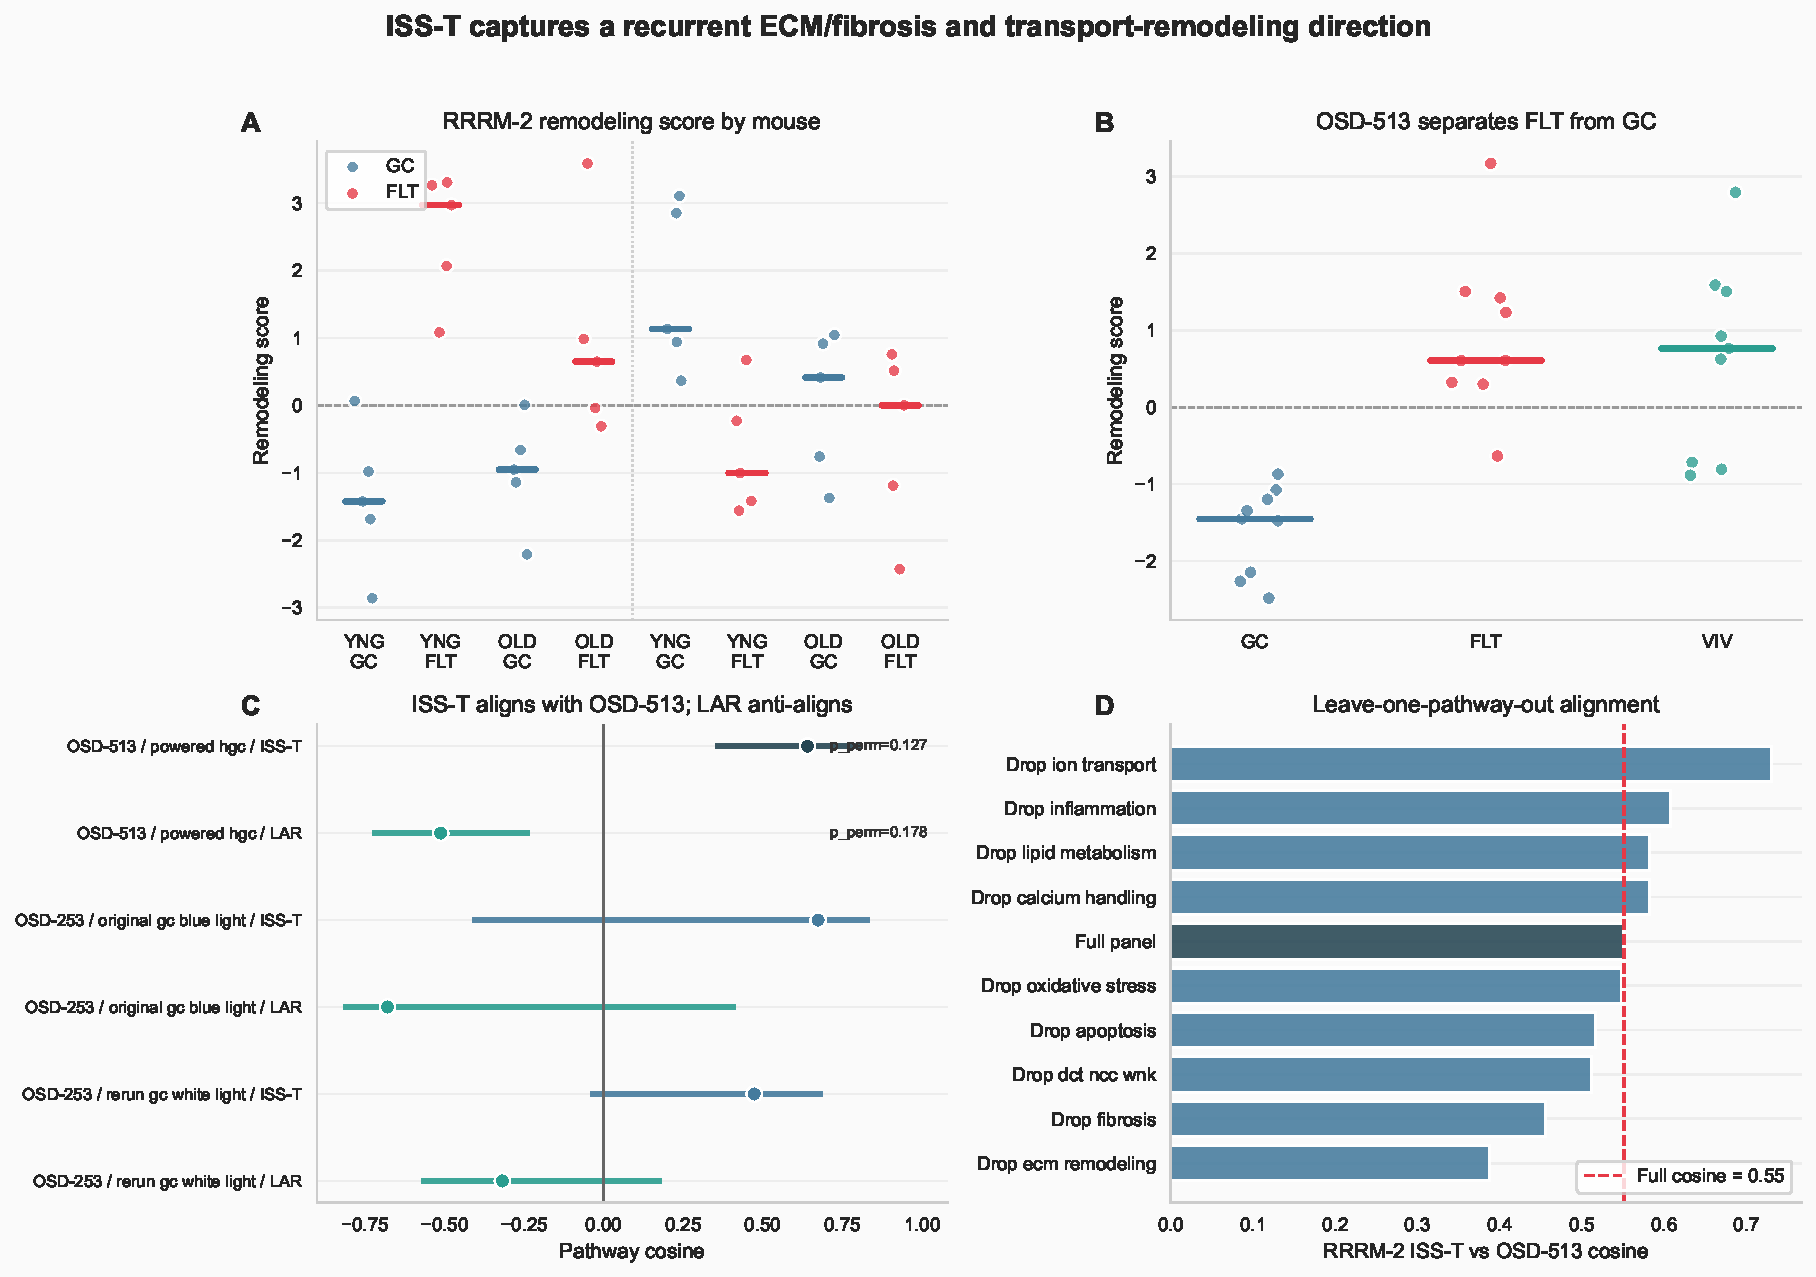
\includegraphics[width=\textwidth]{fig1_main_result_multipanel.pdf}
\caption{\textbf{Main result overview.} RRRM-2 and OSD-513 remodeling scores, cross-OSDR alignment, and leave-one-pathway-out sensitivity.}
\end{figure}

\begin{figure}[H]\centering
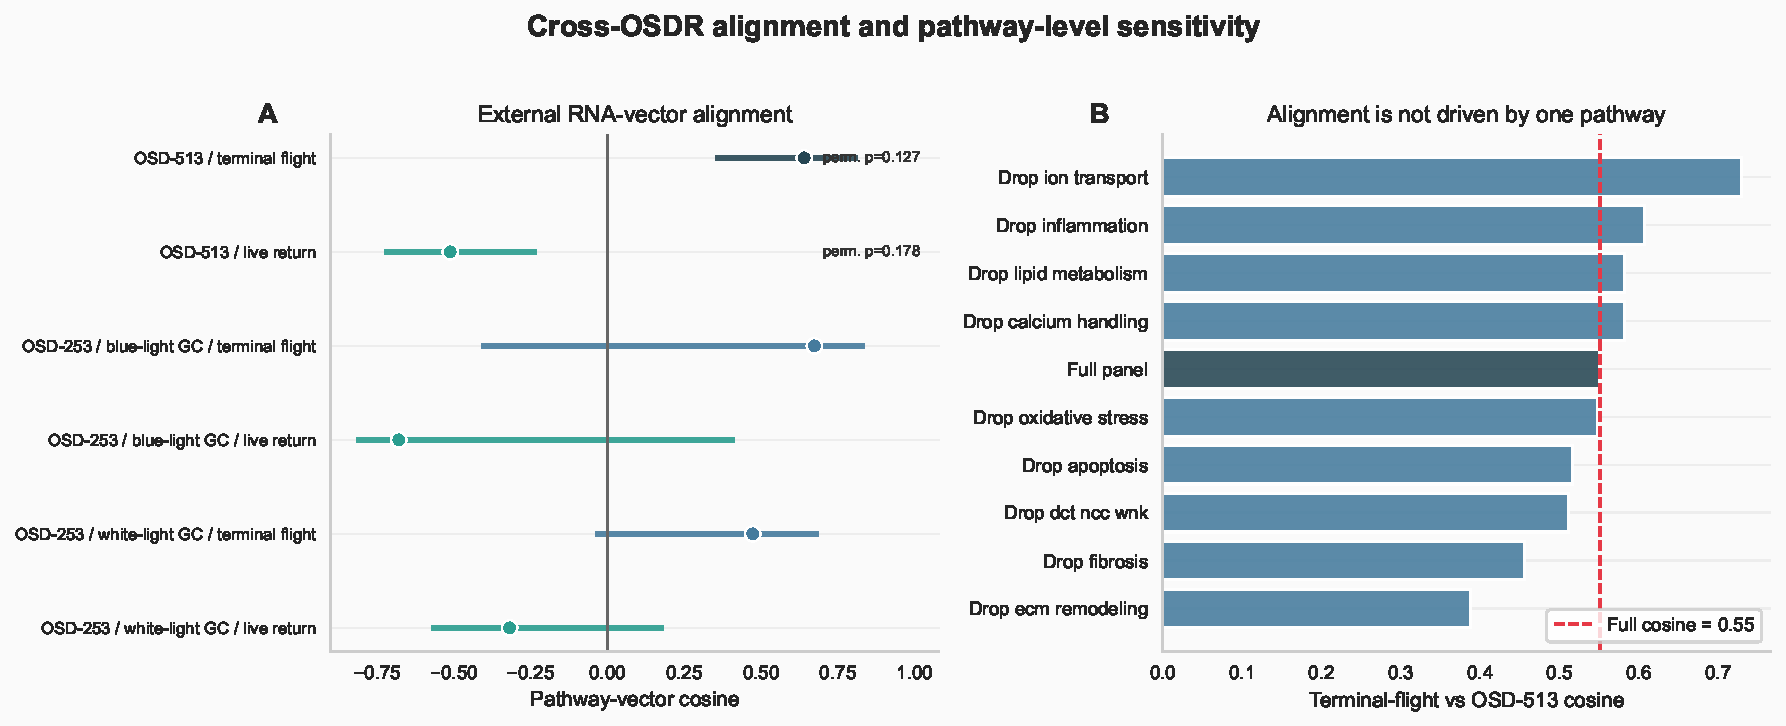
\includegraphics[width=\textwidth]{fig4_cross_alignment_leave_one_out.pdf}
\caption{\textbf{Cross-OSDR alignment and leave-one-pathway-out sensitivity.} ISS-T aligns with OSD-513; LAR is directionally anti-aligned.}
\end{figure}

\begin{figure}[H]\centering
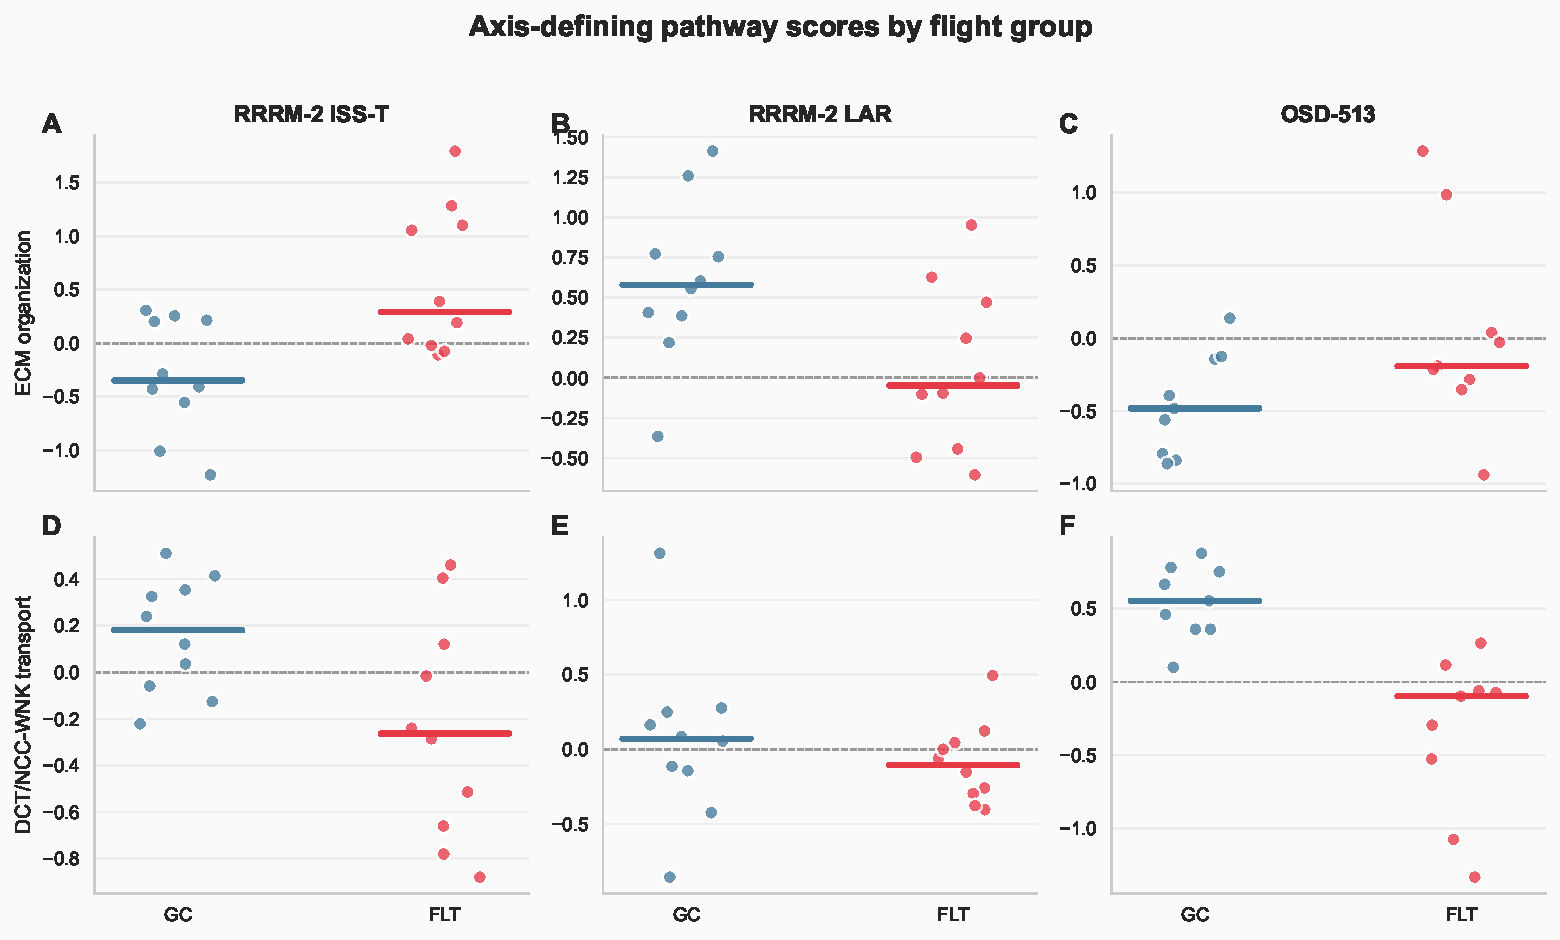
\includegraphics[width=\textwidth]{fig3_pathway_scores_by_flight.pdf}
\caption{\textbf{Axis-defining pathway scores by flight group.} ECM/stromal features rise and DCT/NCC-WNK transport falls in the aligned terminal-flight contexts.}
\end{figure}

\begin{figure}[H]\centering
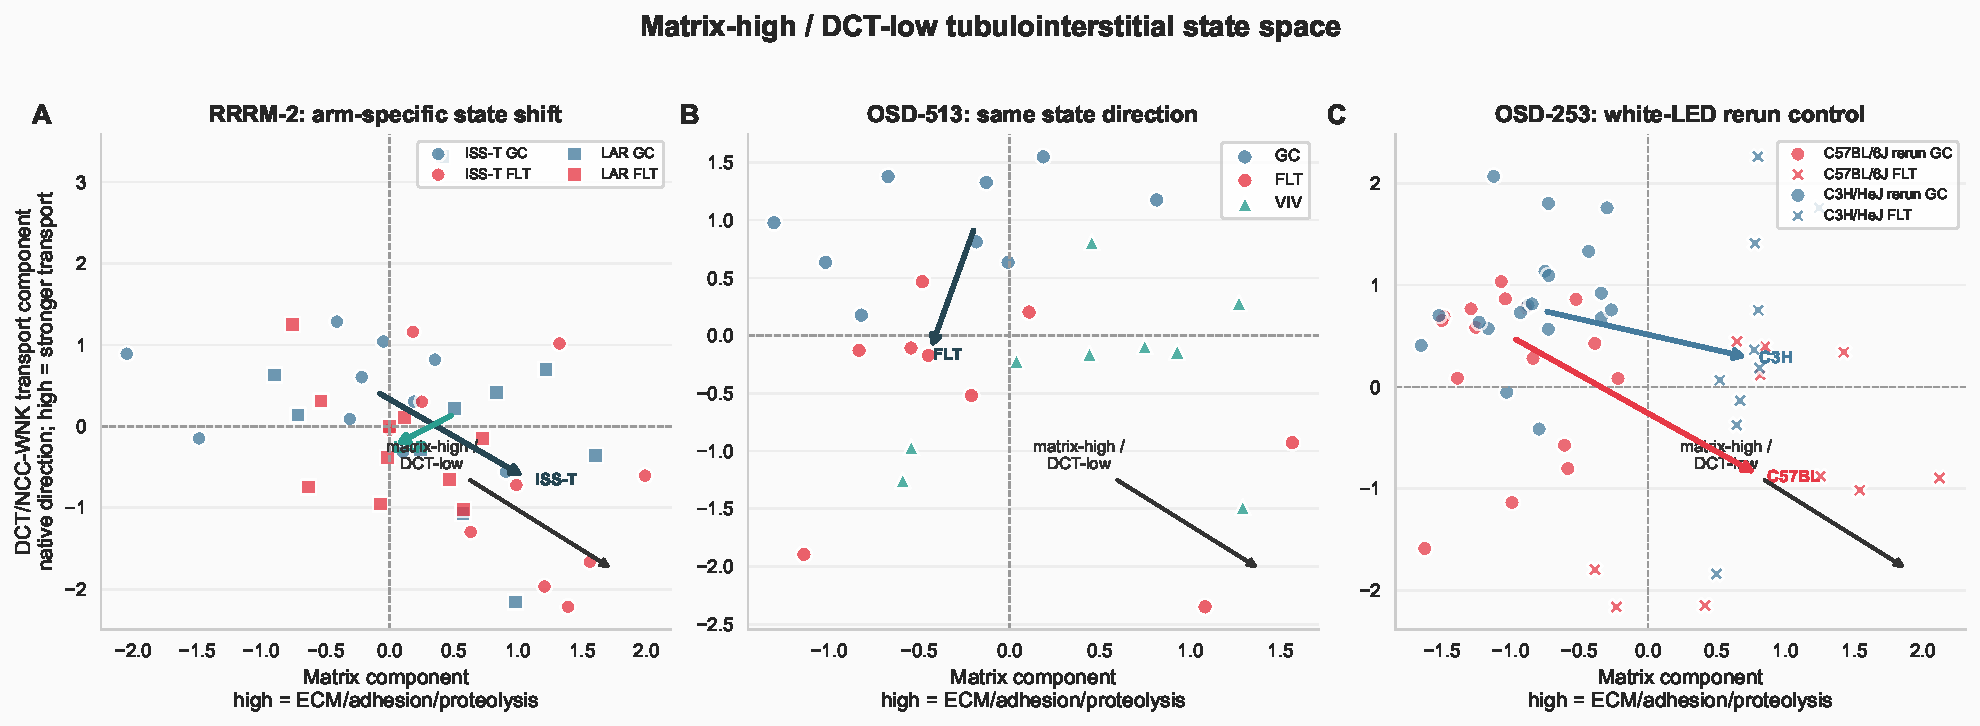
\includegraphics[width=\textwidth]{fig8_tubulointerstitial_state_space.pdf}
\caption{\textbf{DCT/NCC-low state space.} Matrix component on the x-axis, DCT transport in native direction on the y-axis.}
\end{figure}

\begin{figure}[H]\centering
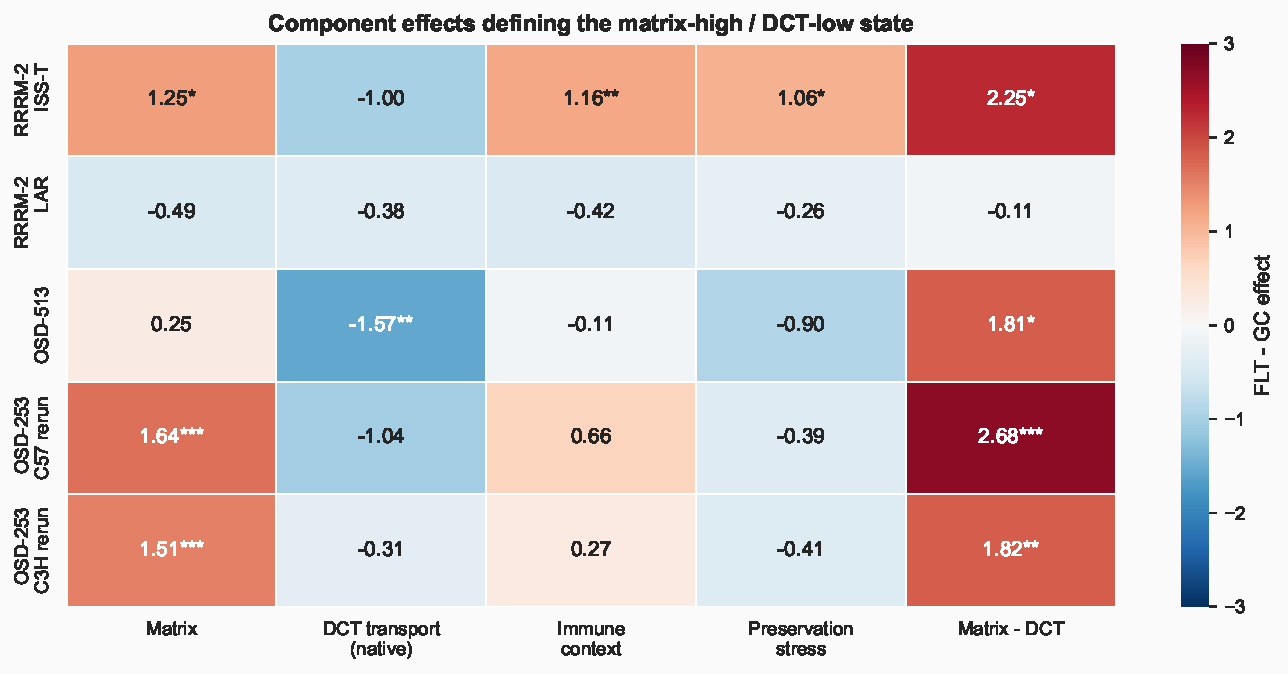
\includegraphics[width=\textwidth]{fig11_state_component_effects.pdf}
\caption{\textbf{State component effects.} FLT-minus-GC effects in standardized component units; DCT transport is shown in native direction.}
\end{figure}

\begin{figure}[H]\centering
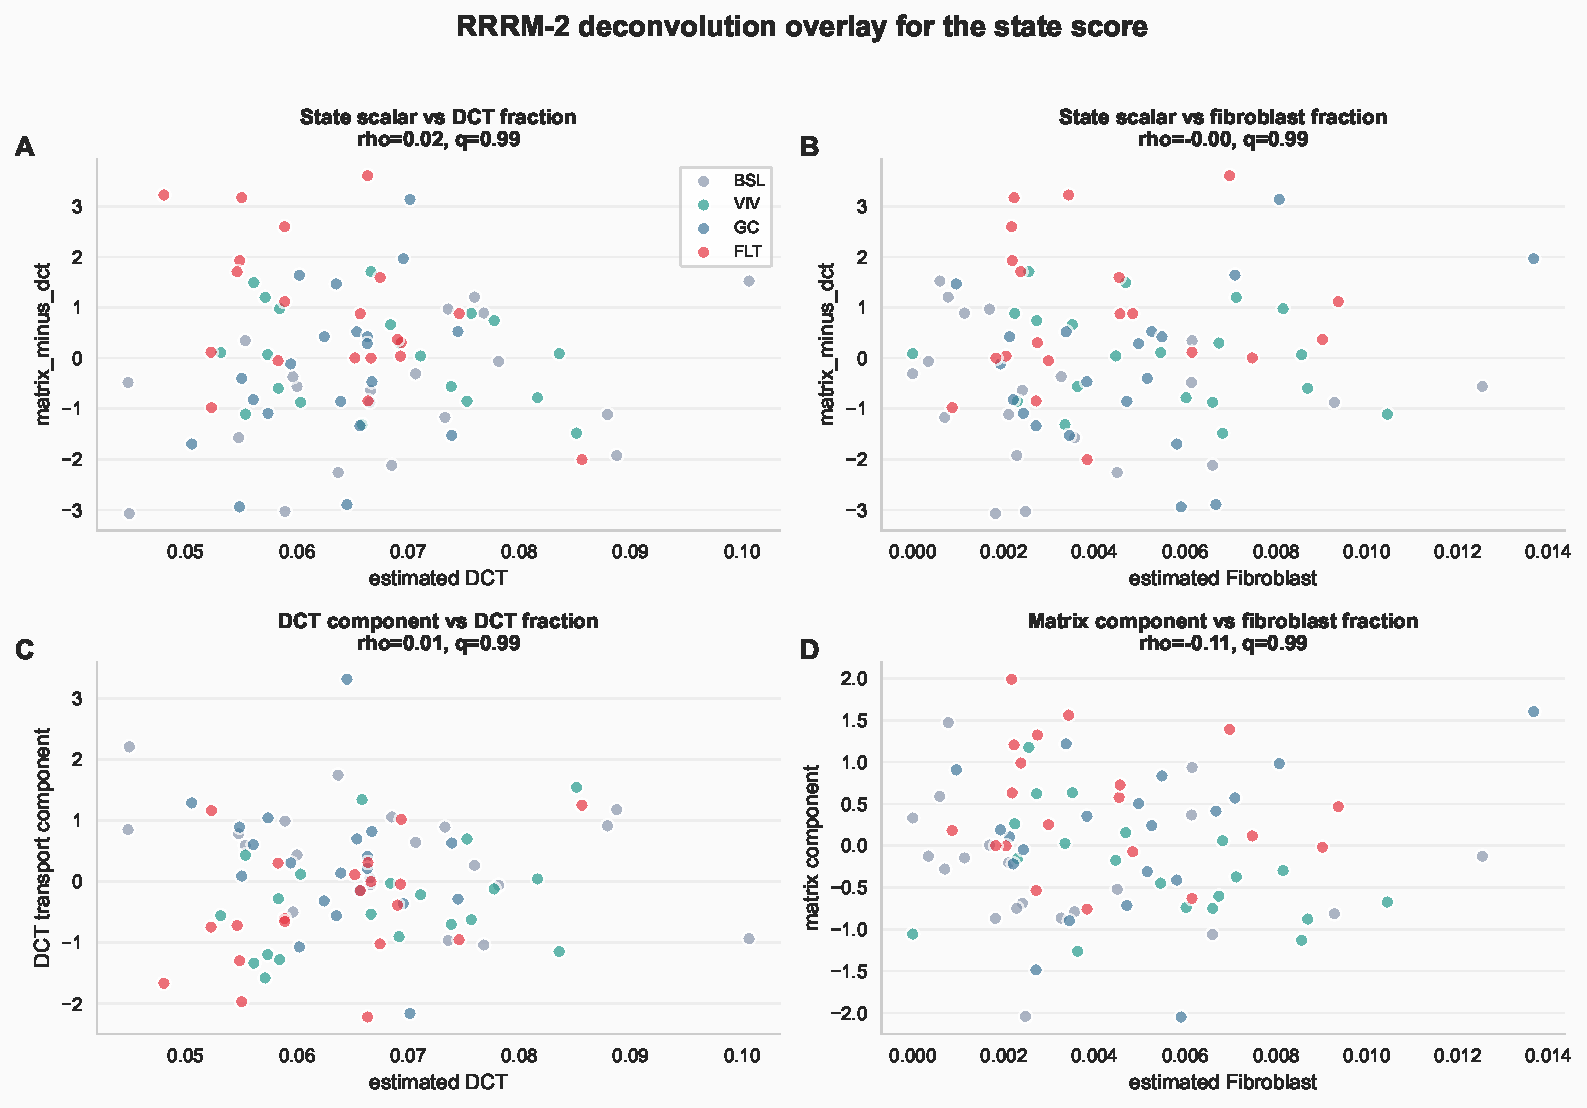
\includegraphics[width=\textwidth]{fig9_rrrm2_deconvolution_overlay.pdf}
\caption{\textbf{RRRM-2 deconvolution overlay.} The state score and components do not reduce to estimated DCT or fibroblast fraction in the available deconvolution model.}
\end{figure}

\begin{figure}[H]\centering
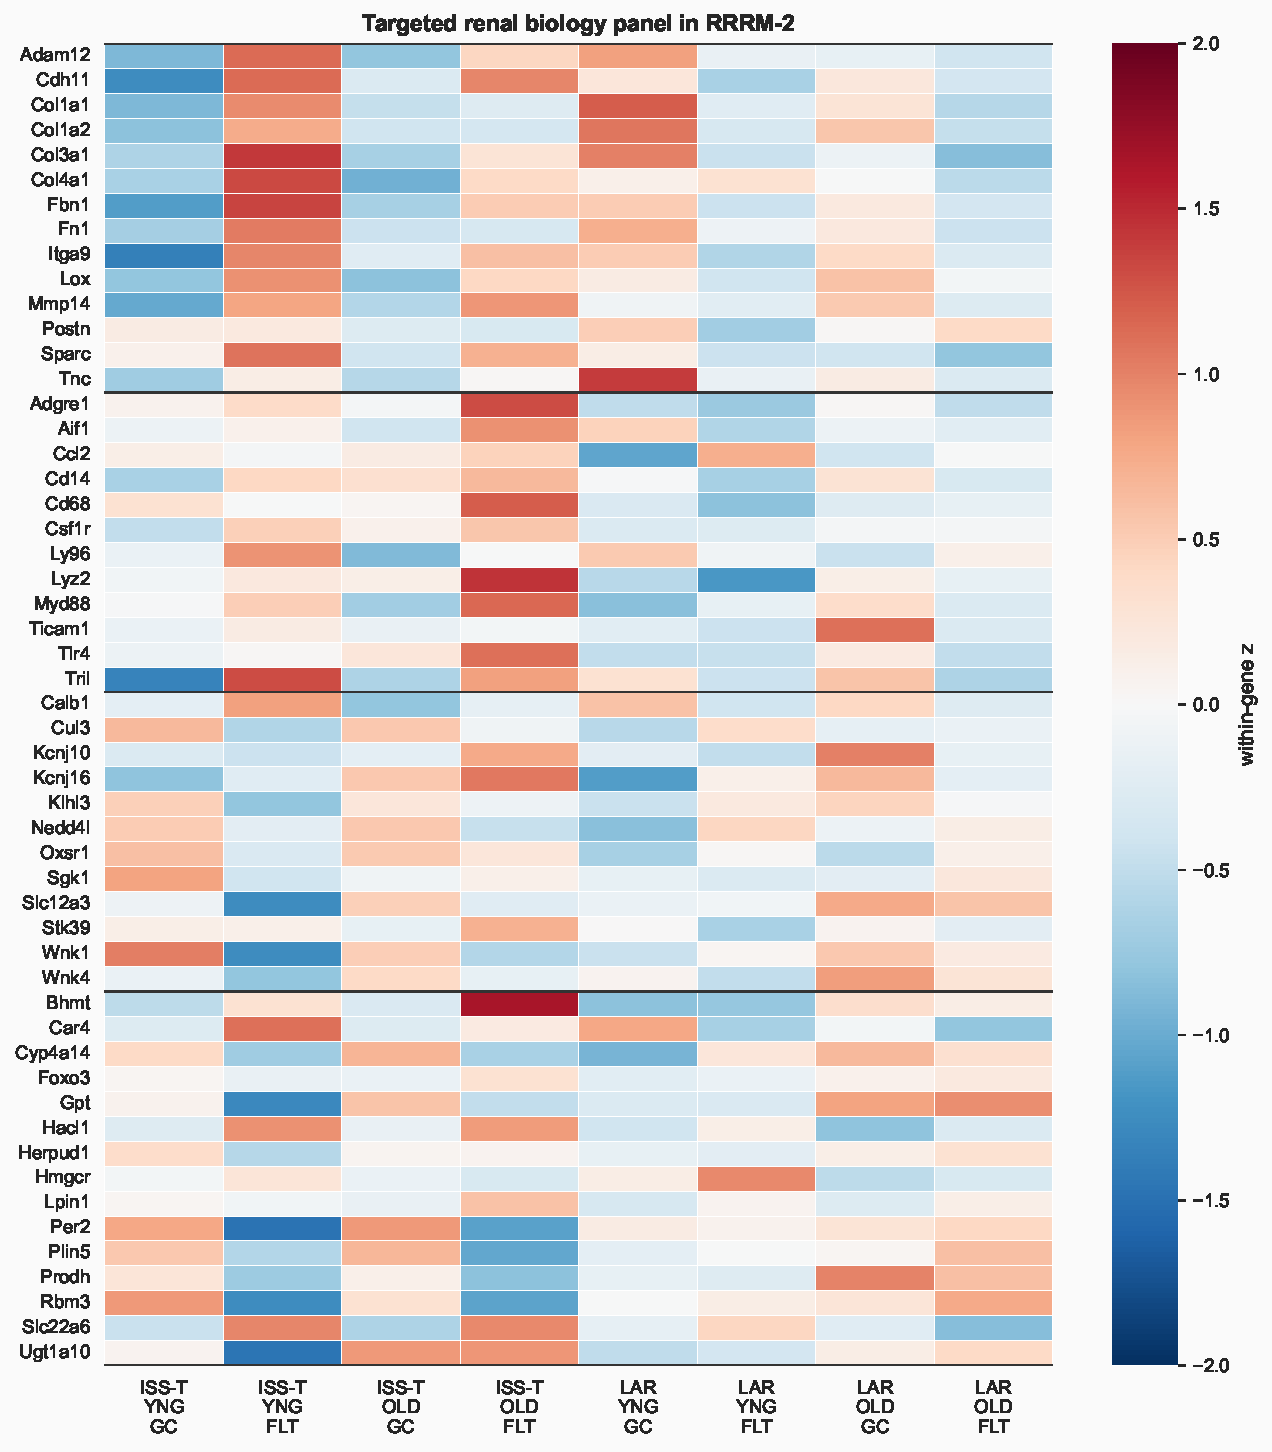
\includegraphics[width=0.95\textwidth]{fig10_targeted_renal_gene_heatmap.pdf}
\caption{\textbf{Targeted renal biology panel.} Residualized RRRM-2 gene expression for ECM/adhesion/proteolysis, innate/macrophage, DCT/NCC-WNK, and tubular/metabolic genes.}
\end{figure}

\begin{figure}[H]\centering
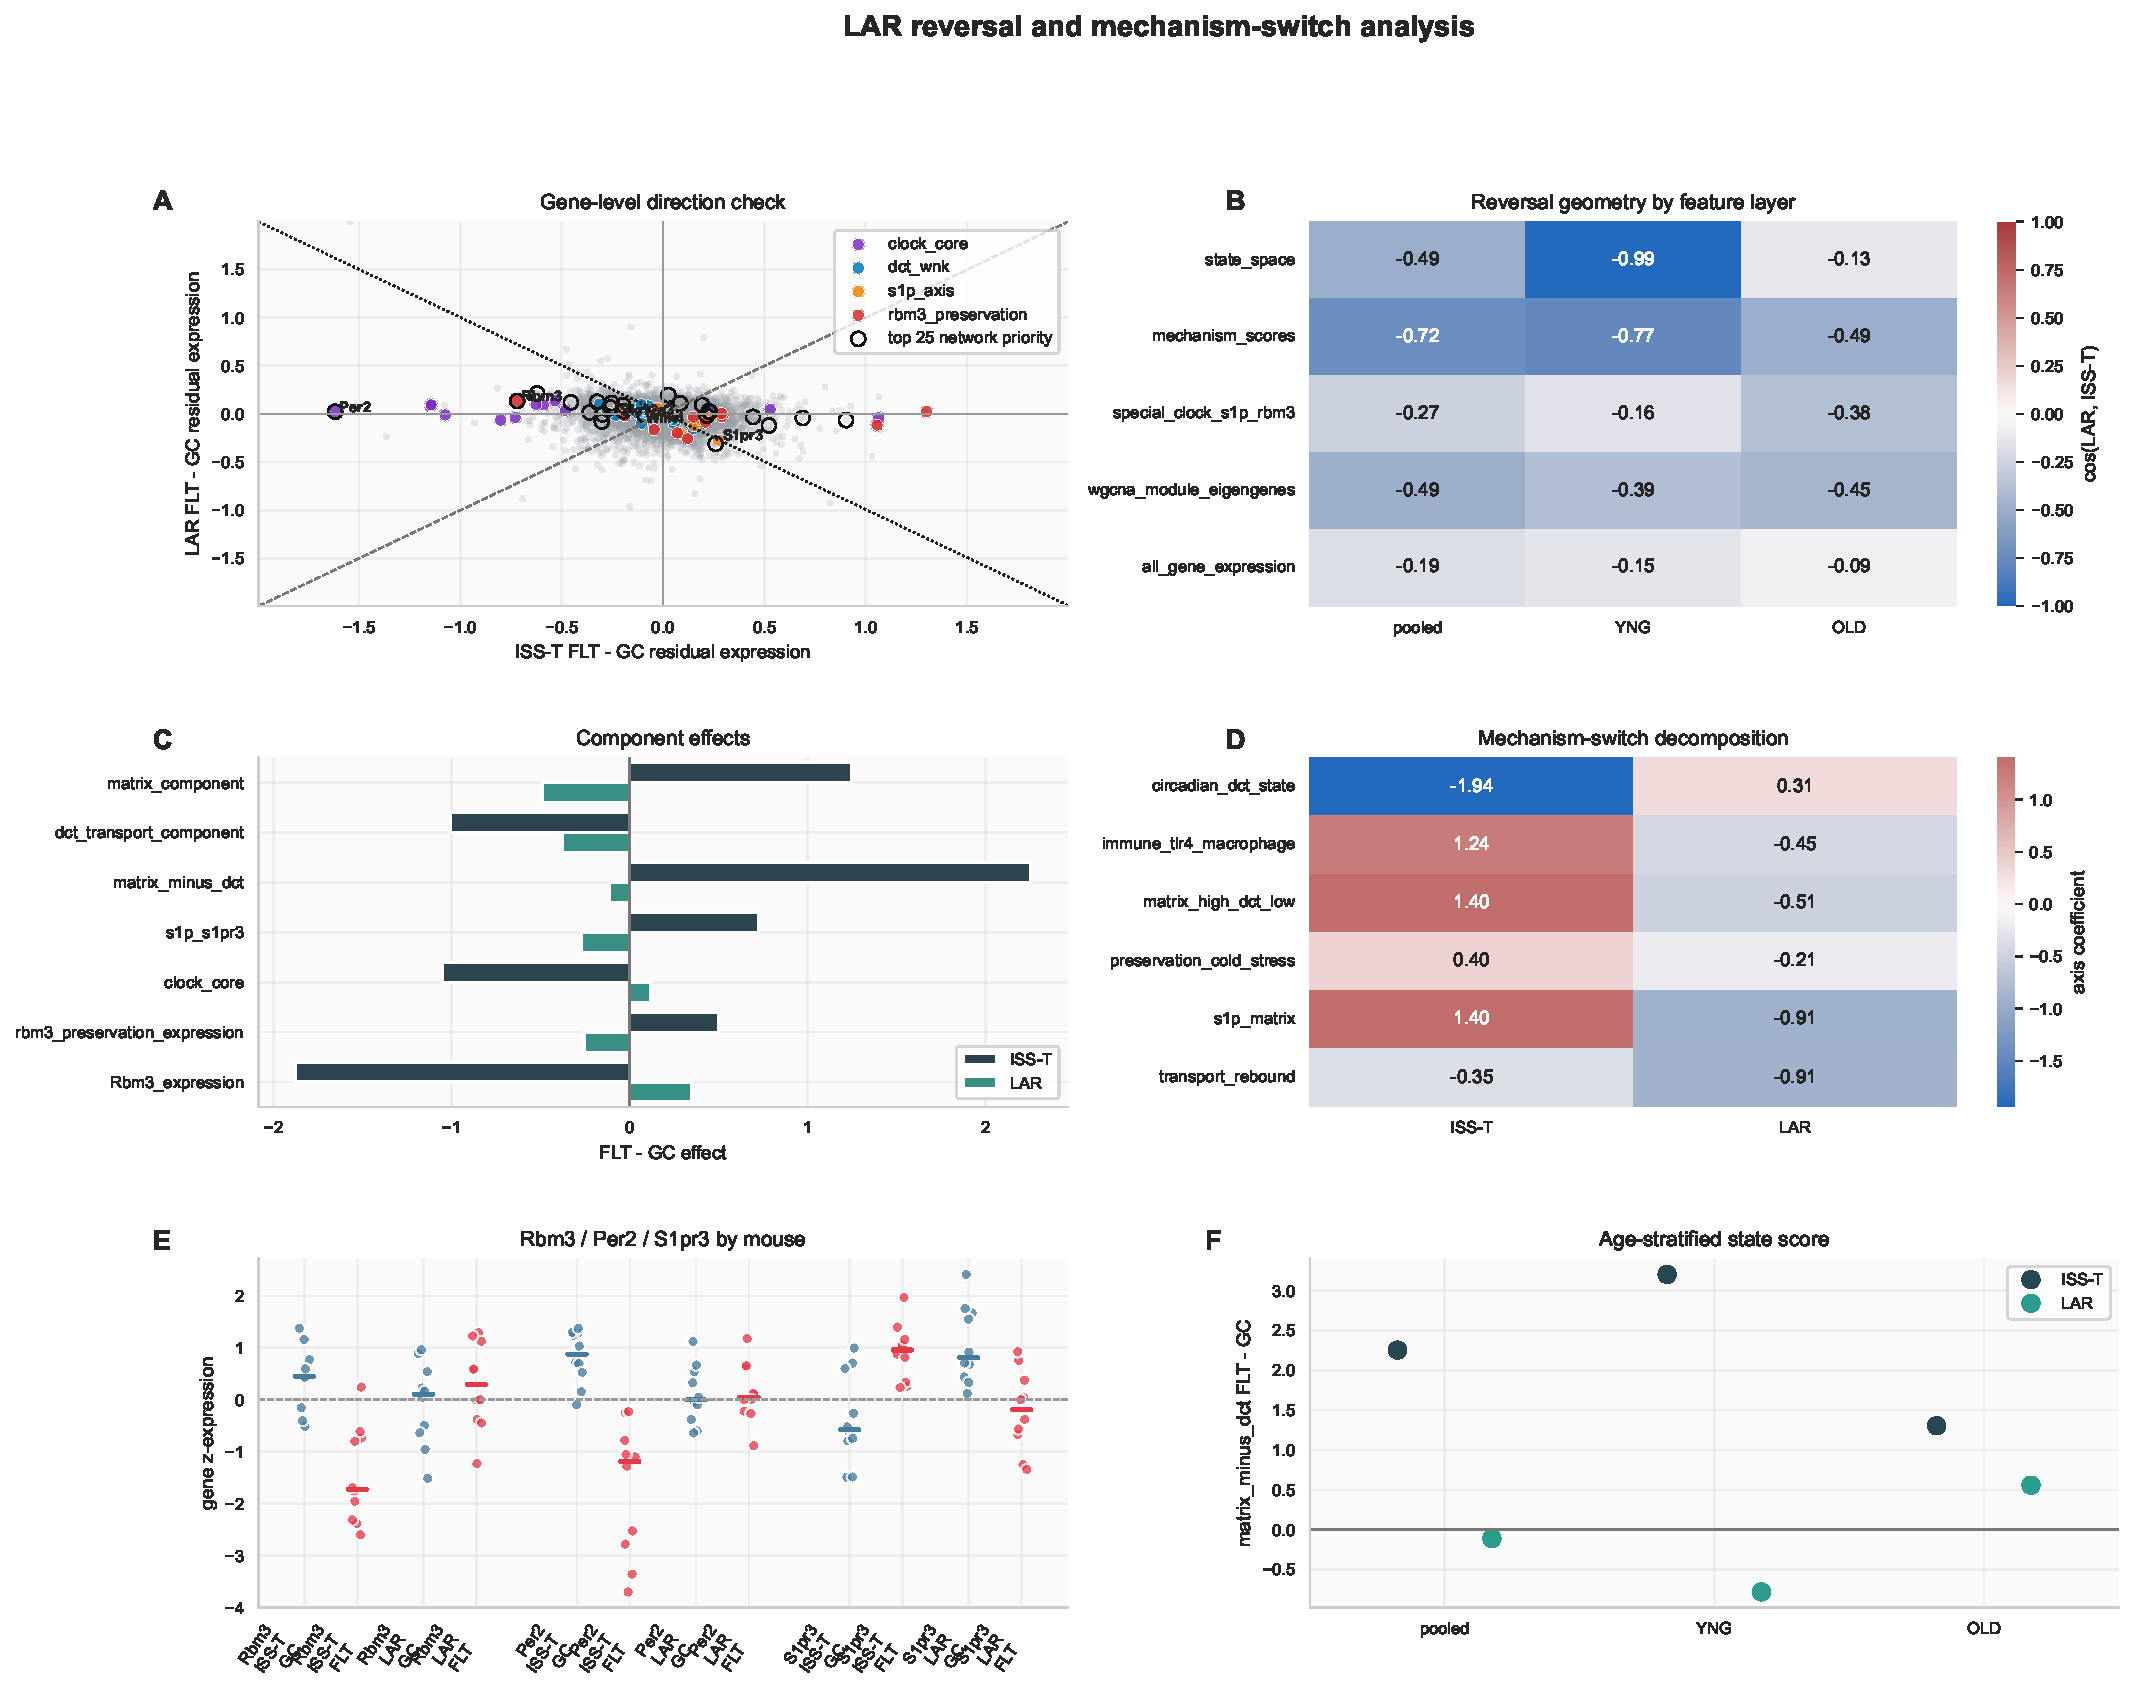
\includegraphics[width=\textwidth]{fig12_lar_reversal_dashboard.pdf}
\caption{\textbf{Live-return arm attenuation/divergence dashboard.} LAR supports attenuation/redirection rather than confirmed reversal.}
\end{figure}

\begin{figure}[H]\centering
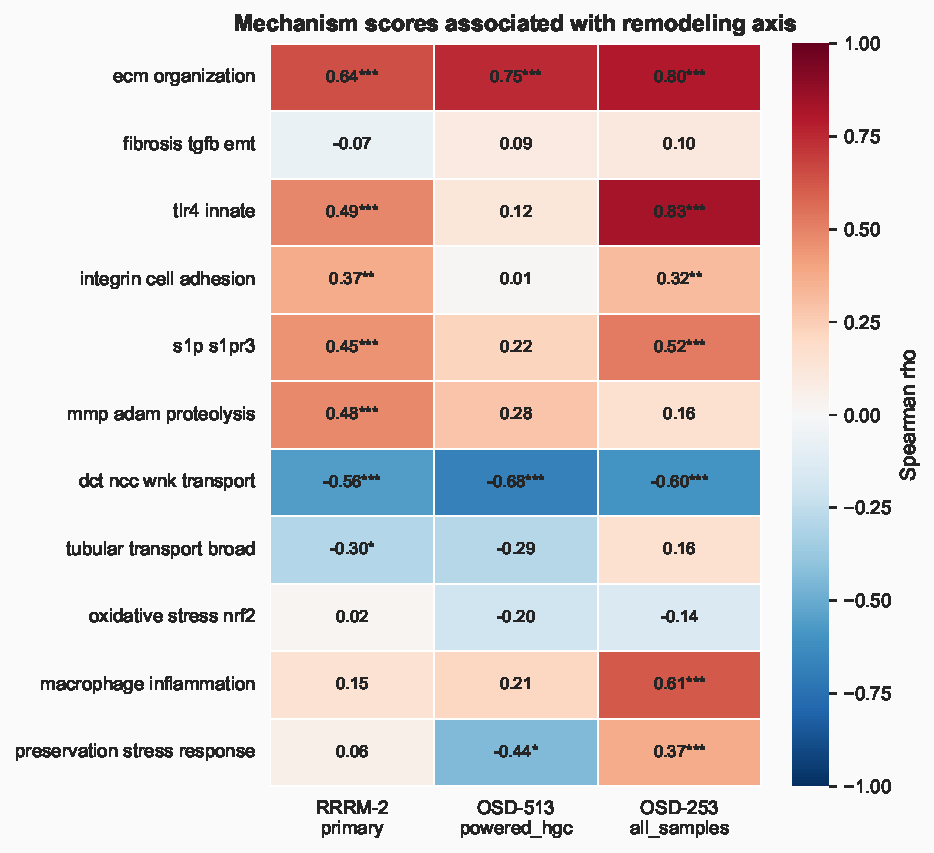
\includegraphics[width=0.82\textwidth]{fig6_mechanism_score_heatmap.pdf}
\caption{\textbf{Mechanism-score associations with the recurrent state} across RRRM-2, OSD-513, and OSD-253.}
\end{figure}

\begin{figure}[H]\centering
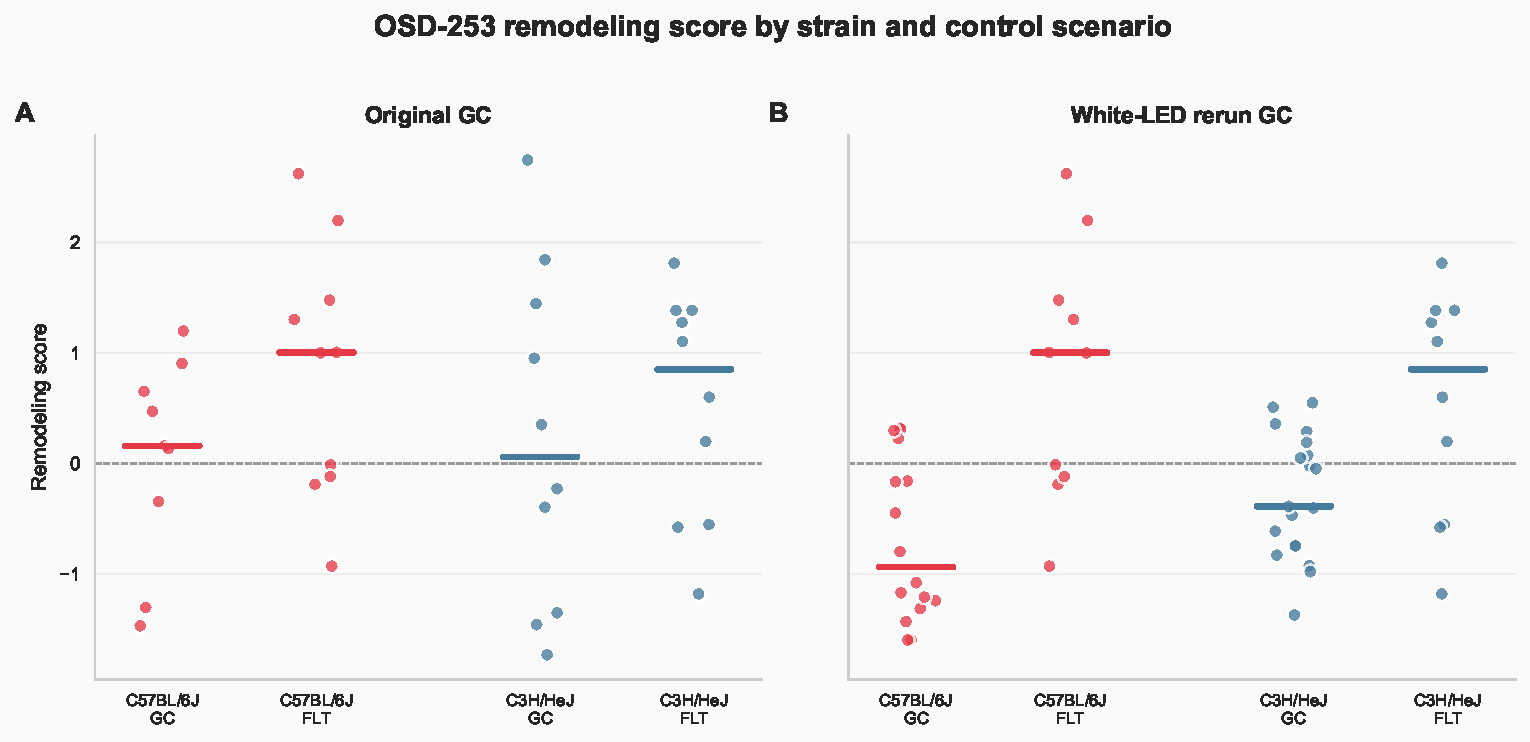
\includegraphics[width=\textwidth]{fig5_osd253_strain_points.pdf}
\caption{\textbf{OSD-253 strain/control-context sensitivity.} C57BL/6J and C3H/HeJ state scores under original and rerun ground-control scenarios.}
\end{figure}

\begin{figure}[H]\centering
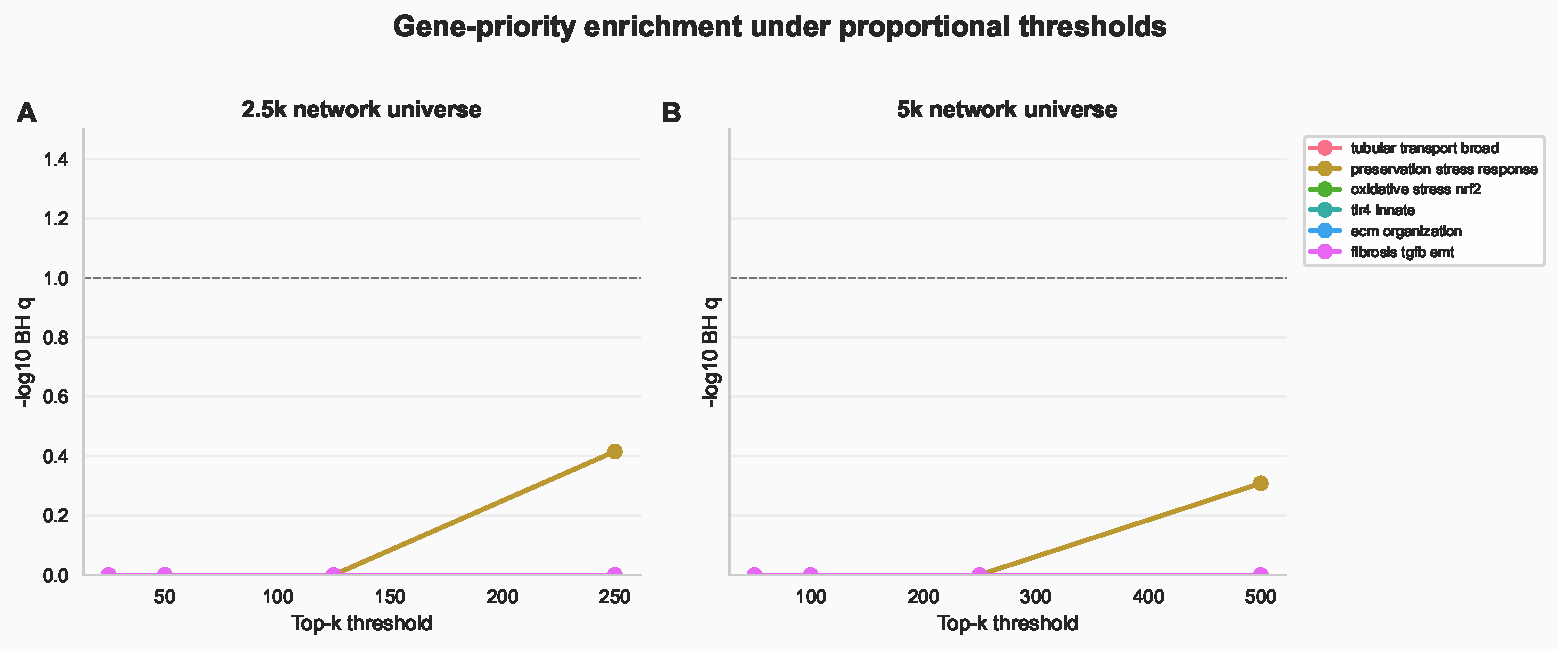
\includegraphics[width=\textwidth]{fig7_gene_priority_sensitivity.pdf}
\caption{\textbf{LIONESS/node2vec gene-priority sensitivity.} Network-prioritized genes provide candidate neighborhoods but do not validate at protein/phosphoprotein level.}
\end{figure}

\begin{figure}[H]\centering
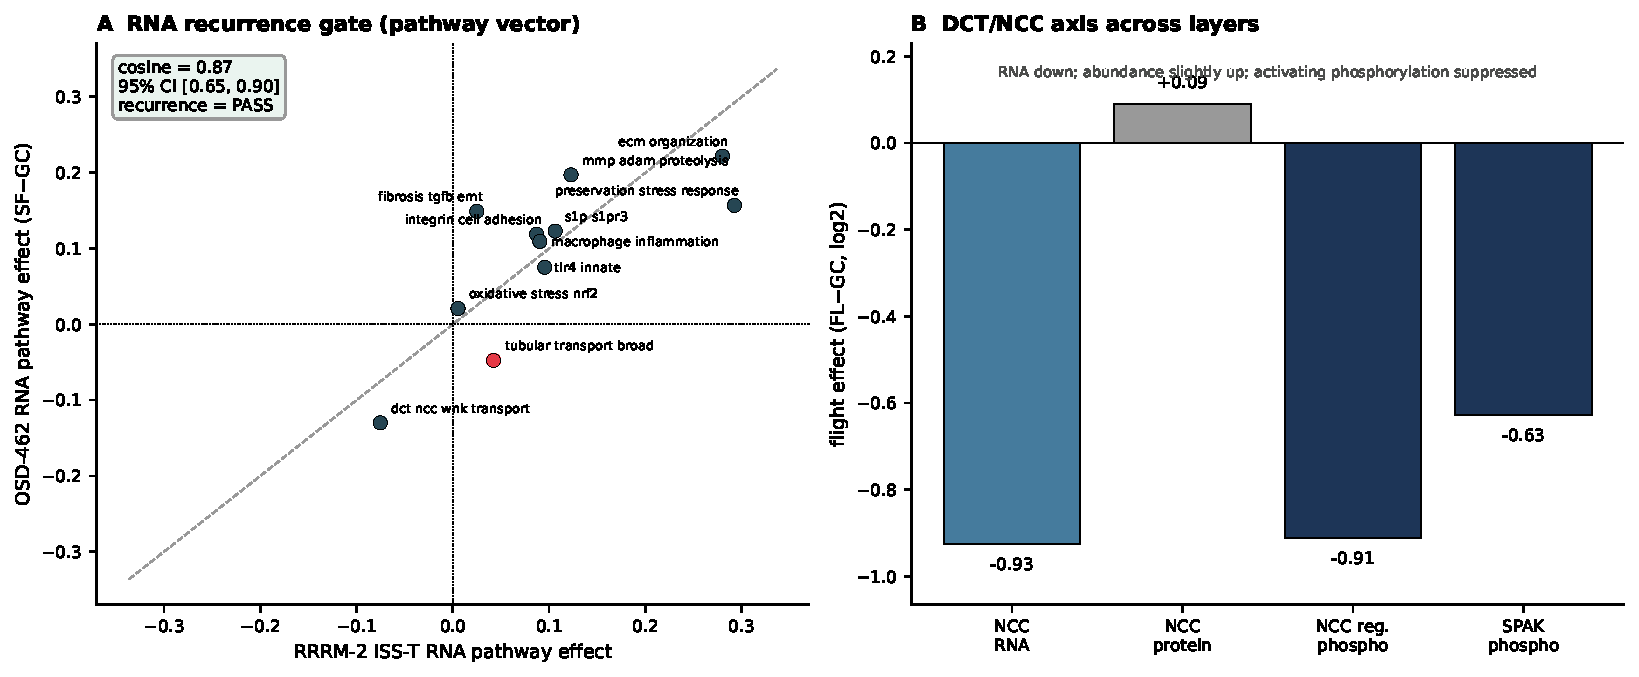
\includegraphics[width=0.9\textwidth]{fig_osd462_rna_recurrence.pdf}
\caption{\textbf{OSD-462 RNA recurrence gate.} OSD-462 RNA reproduces the RRRM-2 ISS-T DCT/NCC-low context direction.}
\end{figure}

\begin{figure}[H]\centering
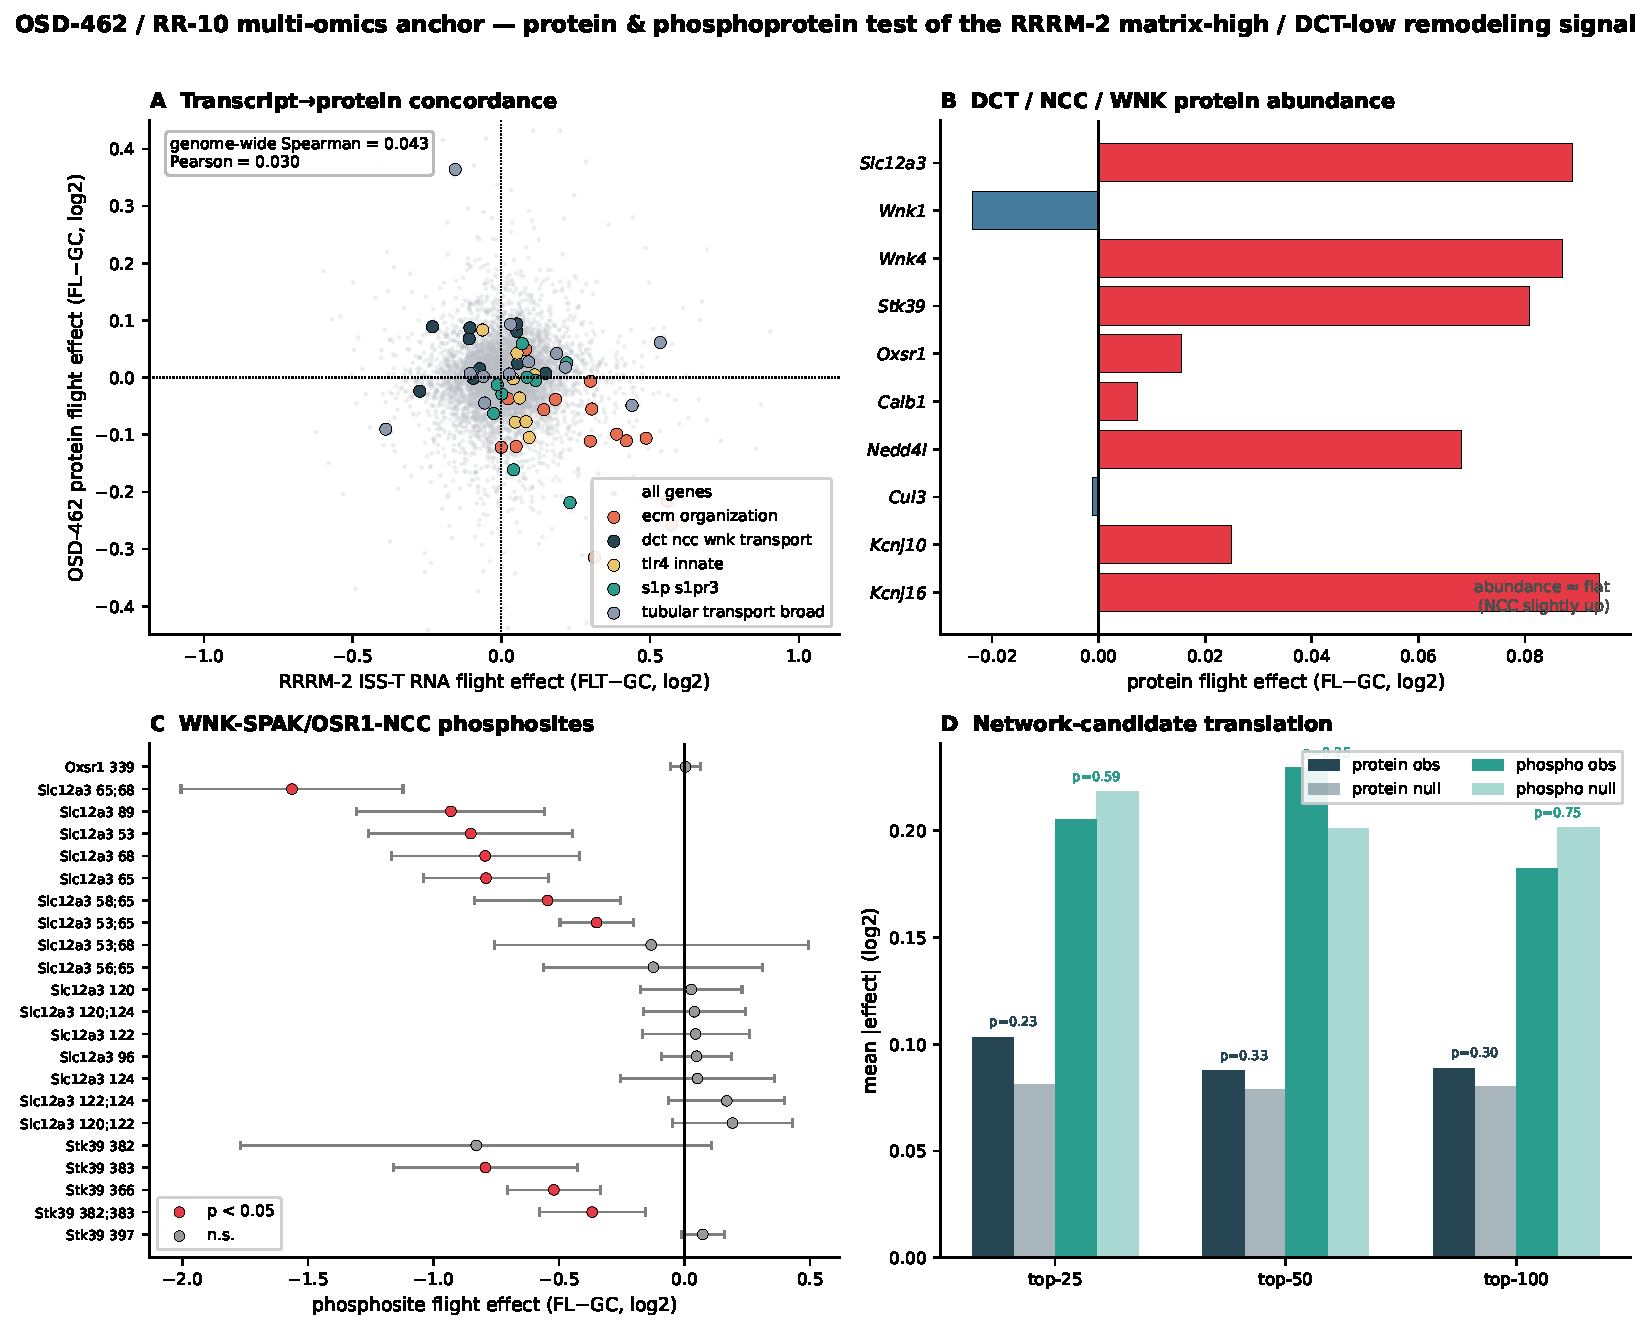
\includegraphics[width=\textwidth]{fig_osd462_multiomics_dashboard.pdf}
\caption{\textbf{OSD-462 multi-omic anchor dashboard.} Transcript-level recurrence, protein-abundance null, and phospho-axis anchoring of the established NCC/SPAK phenotype.}
\end{figure}

\subsection{Secondary and Legacy Curated Figures}

\begin{figure}[H]\centering
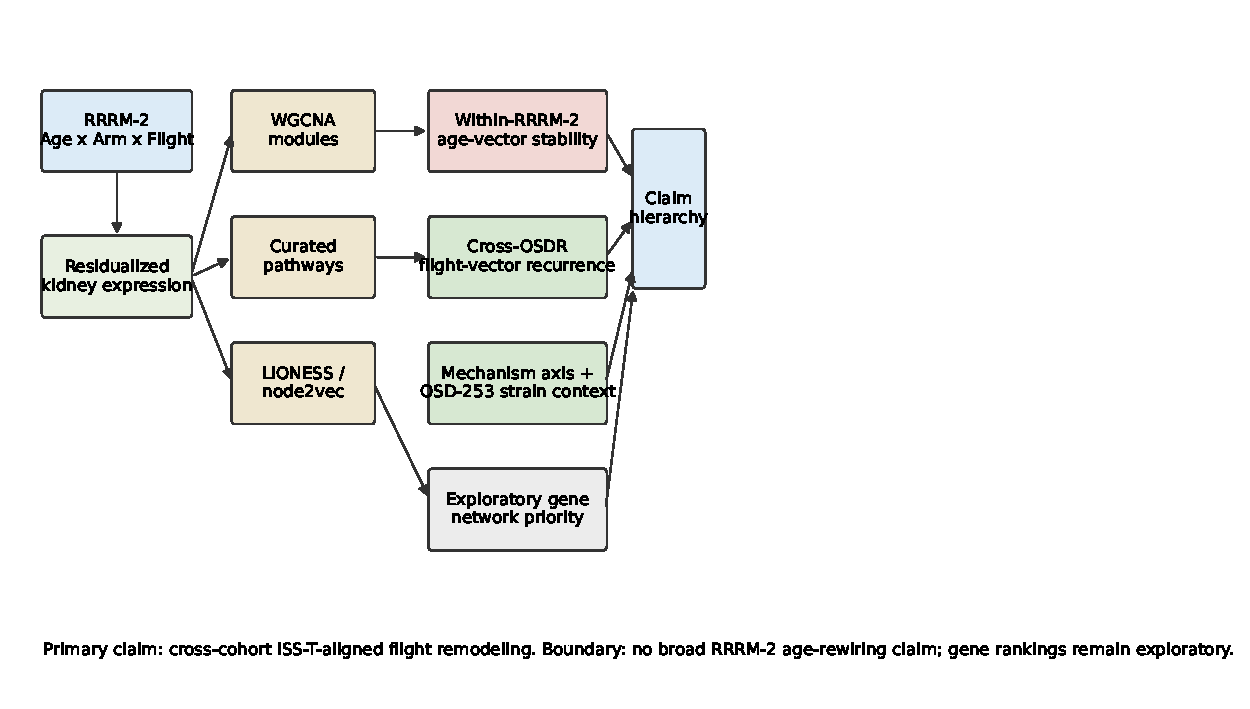
\includegraphics[width=0.95\textwidth]{fig1_workflow_claim_hierarchy.pdf}
\caption{\textbf{Workflow and claim hierarchy.} Analysis layers and claim boundaries used for the state-map manuscript.}
\end{figure}

\begin{figure}[H]\centering
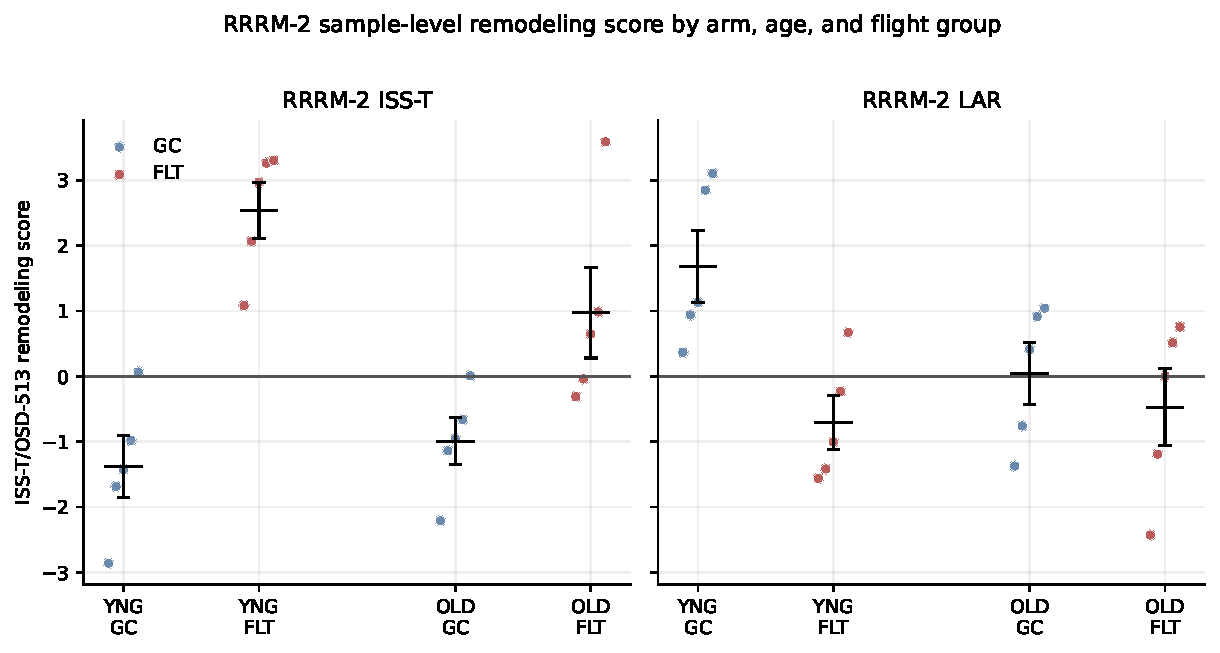
\includegraphics[width=0.95\textwidth]{fig1_rrrm2_remodeling_points.pdf}
\caption{\textbf{RRRM-2 remodeling points.} Earlier standalone view of RRRM-2 remodeling scores by group.}
\end{figure}

\begin{figure}[H]\centering
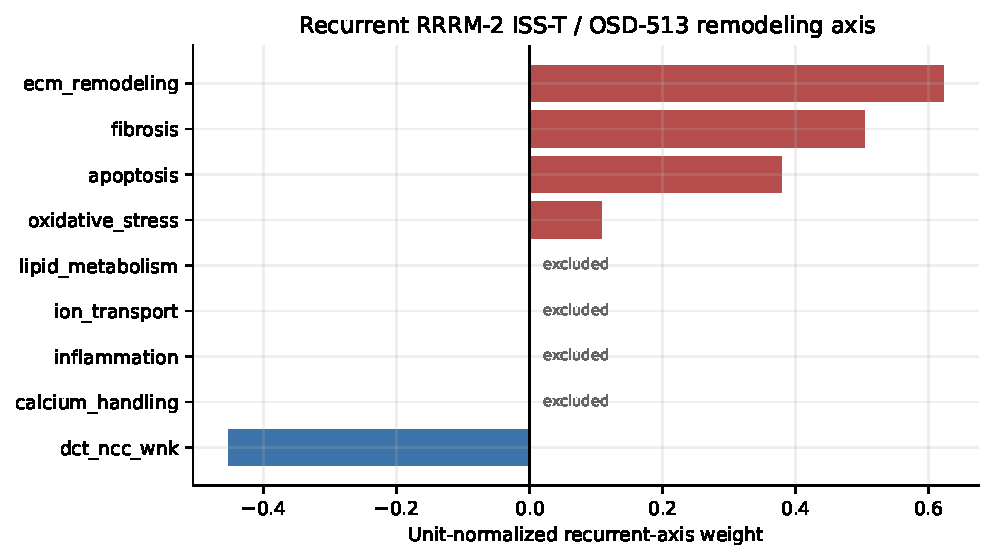
\includegraphics[width=0.95\textwidth]{fig2_recurrent_axis_weights.pdf}
\caption{\textbf{Recurrent-axis weights.} Pathway weights defining the terminal-flight DCT/NCC-low context direction.}
\end{figure}

\begin{figure}[H]\centering
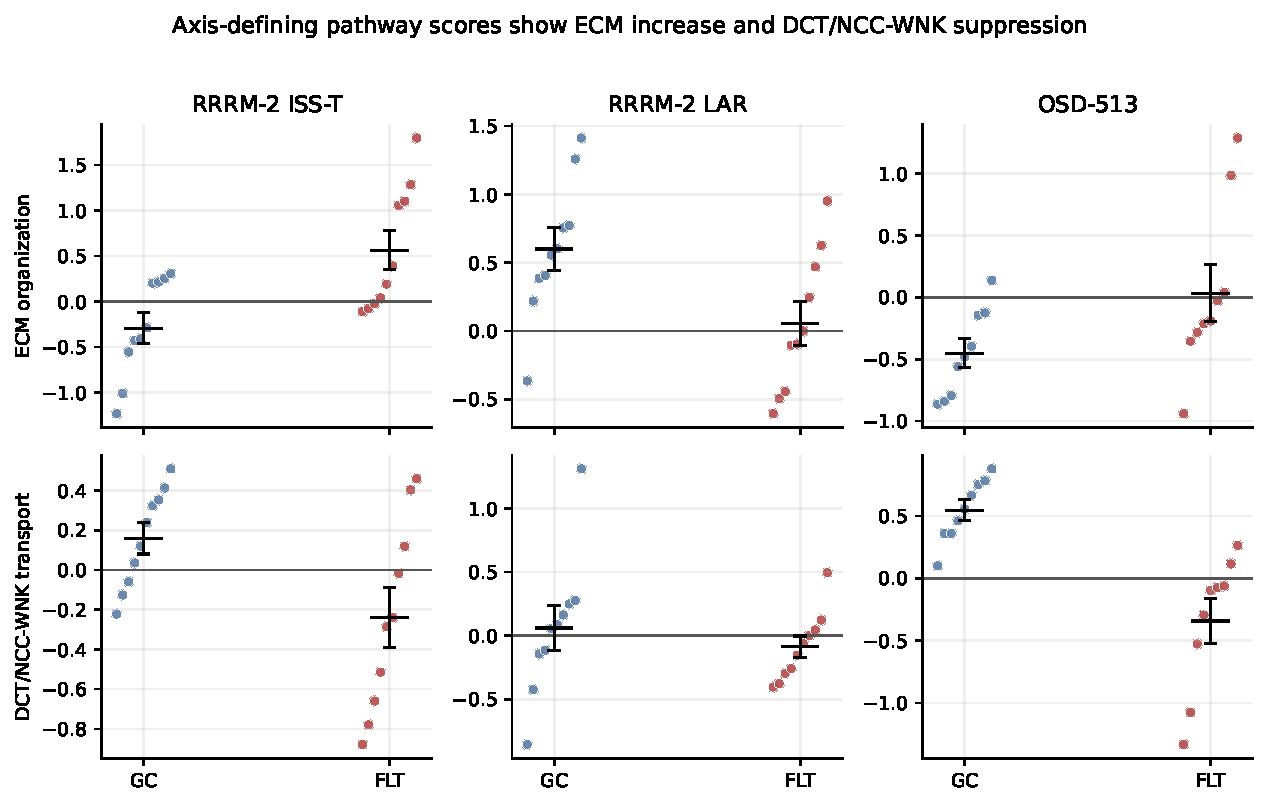
\includegraphics[width=0.95\textwidth]{fig2_pathway_scores_by_flight.pdf}
\caption{\textbf{Pathway scores by flight, alternate numbering.} Earlier figure export retained for completeness.}
\end{figure}

\begin{figure}[H]\centering
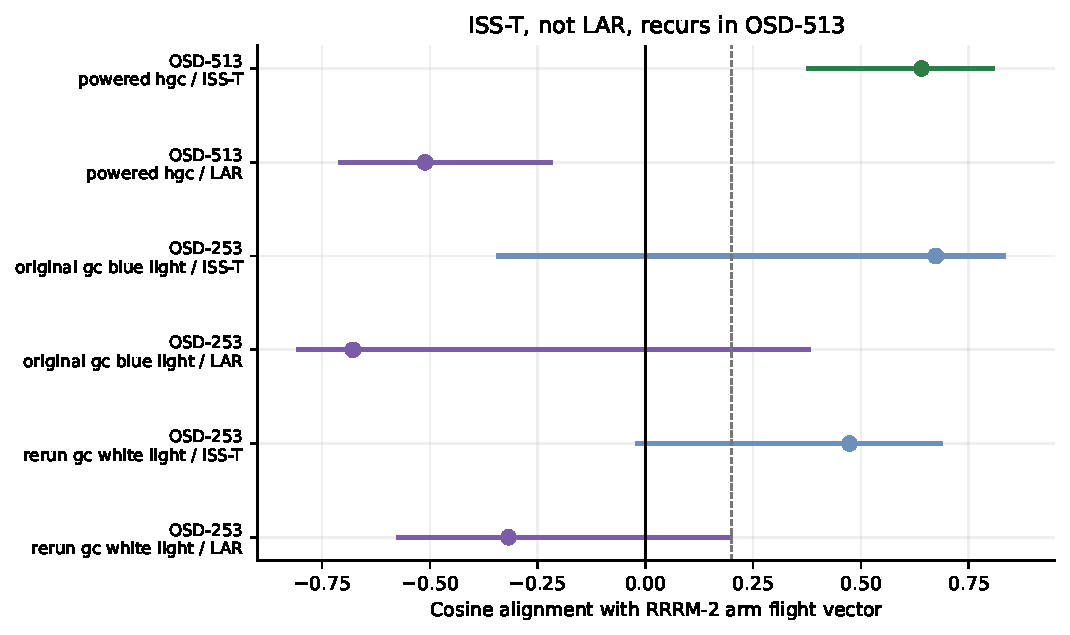
\includegraphics[width=0.95\textwidth]{fig3_cross_osdr_alignment.pdf}
\caption{\textbf{Cross-OSDR alignment, standalone view.} Earlier figure export retained for completeness.}
\end{figure}

\begin{figure}[H]\centering
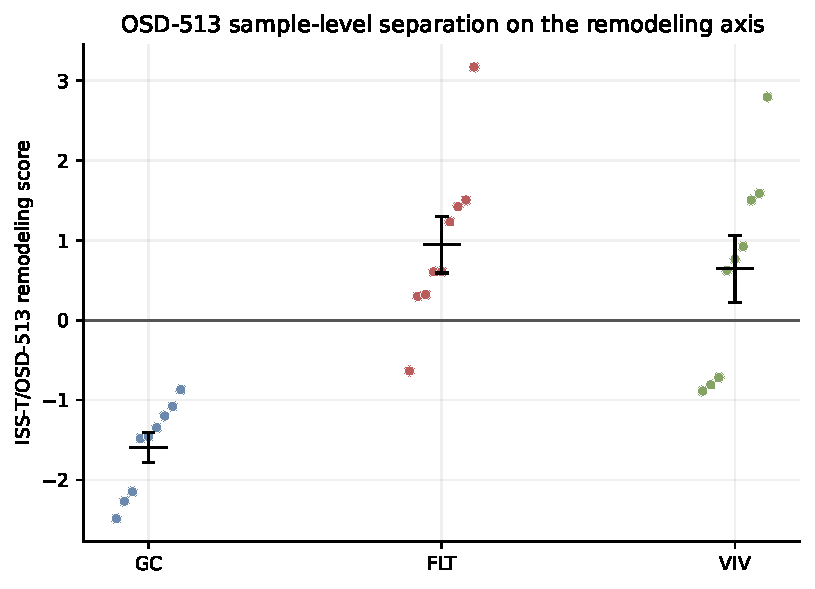
\includegraphics[width=0.95\textwidth]{fig3_osd513_sample_separation.pdf}
\caption{\textbf{OSD-513 sample separation.} Independent kidney cohort state-score separation.}
\end{figure}

\begin{figure}[H]\centering
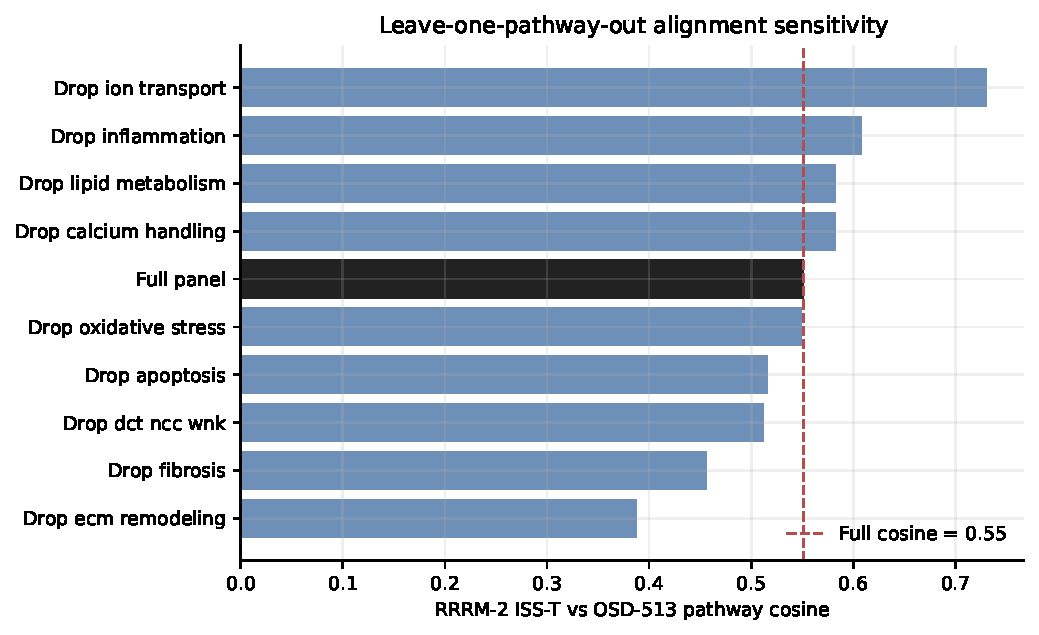
\includegraphics[width=0.95\textwidth]{fig4_leave_one_pathway_out.pdf}
\caption{\textbf{Leave-one-pathway-out sensitivity.} Earlier standalone sensitivity view.}
\end{figure}

\begin{figure}[H]\centering
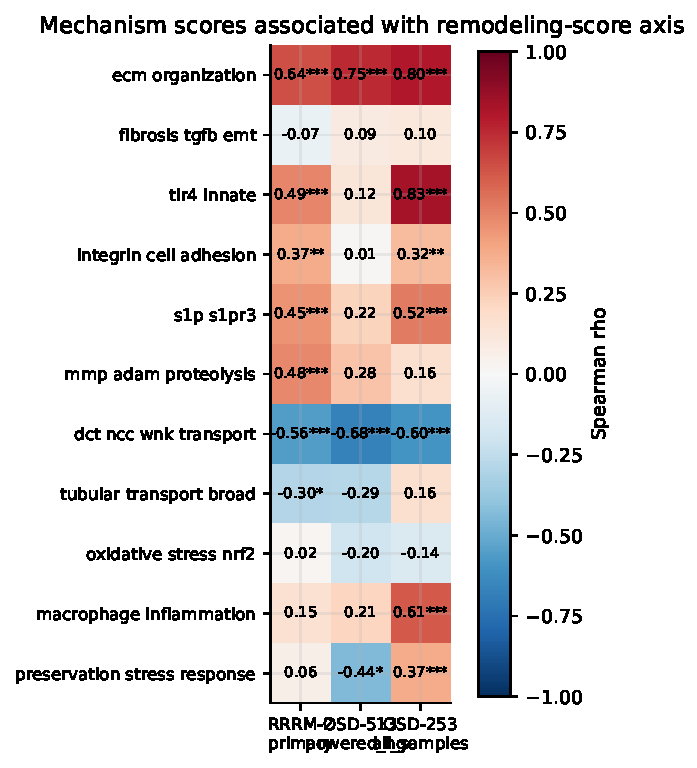
\includegraphics[width=0.95\textwidth]{fig4_mechanism_score_heatmap.pdf}
\caption{\textbf{Mechanism-score heatmap, earlier export.} Retained for completeness.}
\end{figure}

\begin{figure}[H]\centering
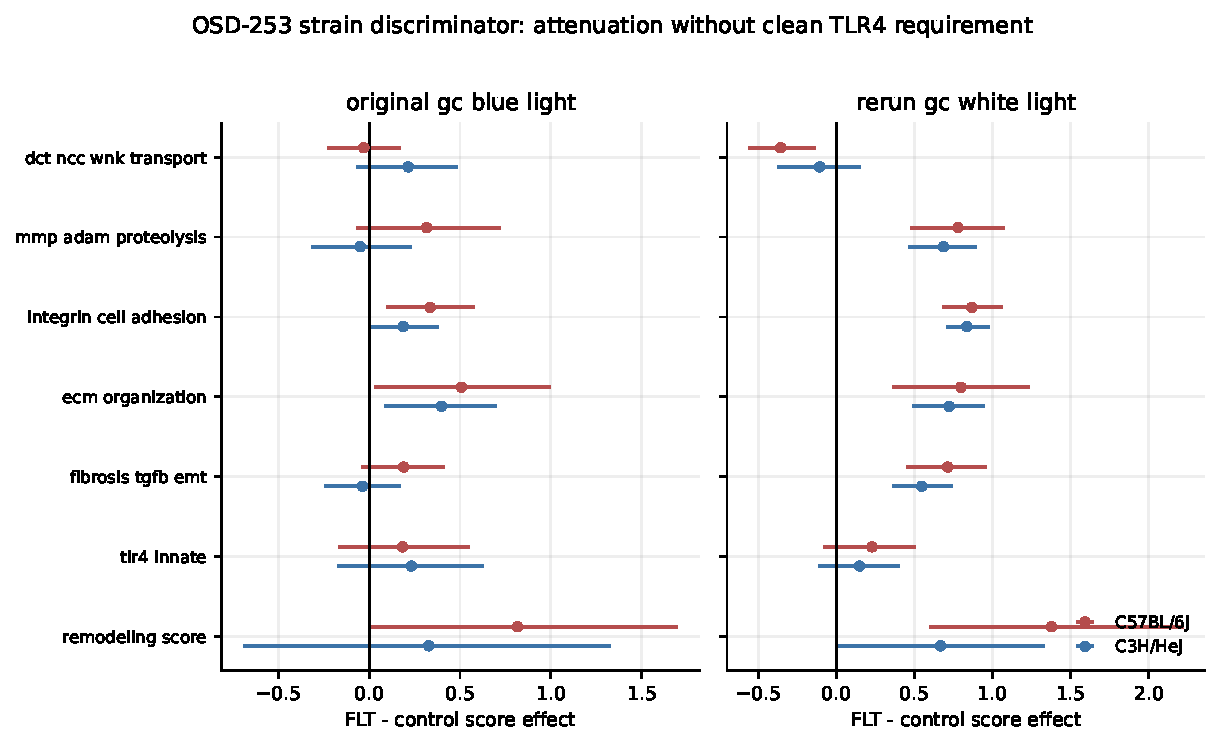
\includegraphics[width=0.95\textwidth]{fig5_osd253_strain_discriminator.pdf}
\caption{\textbf{OSD-253 strain discriminator.} Earlier TLR4/strain-context visualization.}
\end{figure}

\begin{figure}[H]\centering
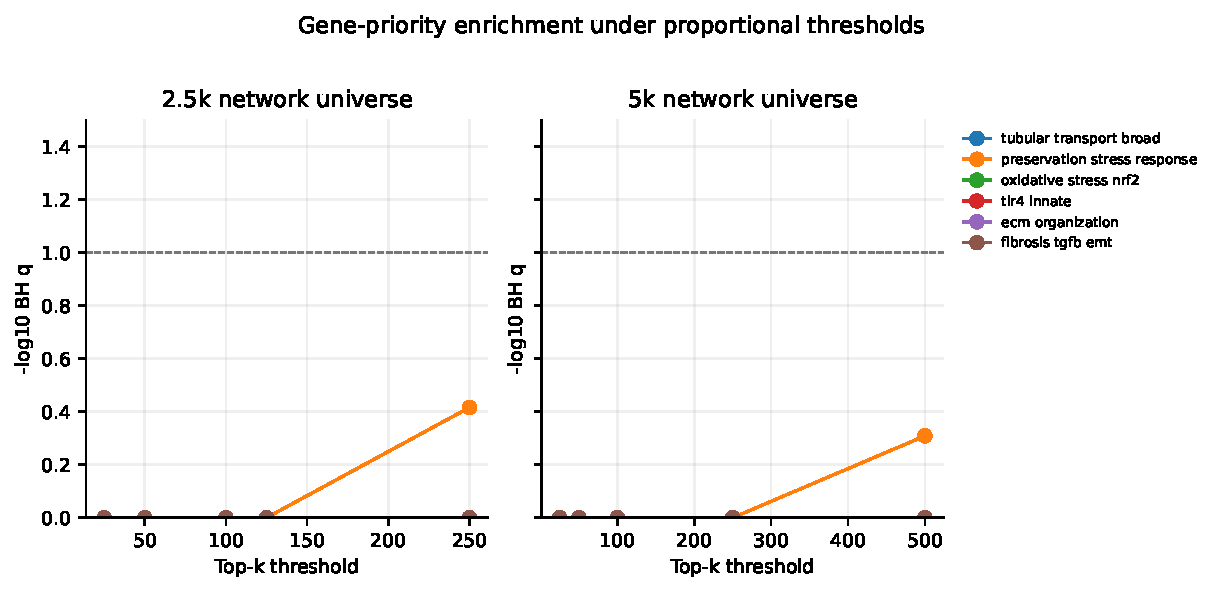
\includegraphics[width=0.95\textwidth]{fig6_gene_priority_sensitivity.pdf}
\caption{\textbf{Gene-priority sensitivity, earlier export.} Retained for completeness.}
\end{figure}

% =====================================================================
\section{Complete Artifact Index}

\begin{longtable}{p{0.30\textwidth}p{0.64\textwidth}}
\caption{\textbf{Complete generated result artifacts indexed by source path.} The compendium embeds the curated manuscript tables and figures above; these files contain the complete machine-readable outputs used to generate them.}\\
\toprule
Category & Complete source artifact(s) \\
\midrule
\endfirsthead
\toprule
Category & Complete source artifact(s) \\
\midrule
\endhead
\bottomrule
\endfoot
Run provenance & \path{data/results/run_20260519_000547_2500g/run_metadata.json}; \path{data/results/run_20260519_cosine_perm_null/run_metadata.json}; \path{data/results/run_20260519_5000g_sensitivity_3seed/run_metadata.json}; \path{data/results/run_20260521_osd462_anchor/osd462_anchor/manifest.json} \\
Age-vector stability & \path{data/results/run_20260519_000547_2500g/contrast_vectors/agc_stability_report.tsv}; \path{data/results/run_20260519_000547_2500g/contrast_vectors/agc_stability_decision.json} \\
Cross-OSDR recurrence & \path{data/results/run_20260519_000547_2500g/contrast_vectors/cross_osdr_recurrence/cross_osdr_alignment_summary.tsv}; \path{data/results/run_20260519_cosine_perm_null/contrast_vectors/cross_osdr_recurrence/*_pathway_permutation.tsv}; \path{data/results/run_20260519_000547_2500g/contrast_vectors/cross_osdr_recurrence/*_pathway_bootstrap.tsv} \\
Recurrent state axis & \path{data/results/run_20260519_000547_2500g/contrast_vectors/mechanism_axis/recurrent_axis_weights.tsv}; \path{data/results/run_20260519_000547_2500g/contrast_vectors/mechanism_axis/sample_remodeling_scores.tsv}; \path{data/results/run_20260519_000547_2500g/contrast_vectors/mechanism_axis/mechanism_score_matrix.tsv} \\
Mechanism context & \path{data/results/run_20260519_000547_2500g/contrast_vectors/mechanism_axis/mechanism_convergence_summary.tsv}; \path{data/results/run_20260519_000547_2500g/contrast_vectors/mechanism_axis/mechanism_score_associations.tsv}; \path{data/results/run_20260519_000547_2500g/contrast_vectors/mechanism_axis/mechanism_gene_set_coverage.tsv}; \path{data/results/run_20260519_000547_2500g/contrast_vectors/mechanism_axis/axis_gene_set_coverage.tsv} \\
State space & \path{data/results/run_20260519_000547_2500g/contrast_vectors/mechanism_axis/tubulointerstitial_state/state_space_scores.tsv}; \path{data/results/run_20260519_000547_2500g/contrast_vectors/mechanism_axis/tubulointerstitial_state/state_space_group_effects.tsv}; \path{data/results/run_20260519_000547_2500g/contrast_vectors/mechanism_axis/tubulointerstitial_state/state_space_component_correlations.tsv}; \path{data/results/run_20260519_000547_2500g/contrast_vectors/mechanism_axis/tubulointerstitial_state/targeted_renal_gene_panel.tsv} \\
LAR attenuation/divergence & \path{data/results/run_20260519_000547_2500g/contrast_vectors/mechanism_axis/tubulointerstitial_state/lar_reversal/lar_reversal_vector_summary.tsv}; \path{data/results/run_20260519_000547_2500g/contrast_vectors/mechanism_axis/tubulointerstitial_state/lar_reversal/lar_reversal_component_effects.tsv}; \path{data/results/run_20260519_000547_2500g/contrast_vectors/mechanism_axis/tubulointerstitial_state/lar_reversal/lar_reversal_model_calls.tsv}; \path{data/results/run_20260519_000547_2500g/contrast_vectors/mechanism_axis/tubulointerstitial_state/lar_reversal/lar_s1p_axis_analysis.tsv}; \path{data/results/run_20260519_000547_2500g/contrast_vectors/mechanism_axis/tubulointerstitial_state/lar_reversal/lar_circadian_dct_analysis.tsv}; \path{data/results/run_20260519_000547_2500g/contrast_vectors/mechanism_axis/tubulointerstitial_state/lar_reversal/lar_rbm3_preservation_analysis.tsv} \\
OSD-253 strain/TLR4 context & \path{data/results/run_20260519_000547_2500g/contrast_vectors/mechanism_axis/osd253_tlr4_discriminator.tsv}; \path{data/results/run_20260519_000547_2500g/contrast_vectors/mechanism_axis/osd253_tlr4_discriminator_bootstrap.tsv} \\
Gene/network priority & \path{data/results/run_20260519_000547_2500g/contrast_vectors/mechanism_axis/gene_axis_priority.tsv}; \path{data/results/run_20260519_000547_2500g/contrast_vectors/mechanism_axis/gene_axis_priority_top25.tsv}; \path{data/results/run_20260519_000547_2500g/contrast_vectors/mechanism_axis/gene_axis_priority_top50.tsv}; \path{data/results/run_20260519_000547_2500g/contrast_vectors/mechanism_axis/gene_axis_priority_top100.tsv}; \path{data/results/run_20260519_000547_2500g/contrast_vectors/mechanism_axis/gene_priority_enrichment_topk.tsv}; \path{data/results/run_20260519_000547_2500g/contrast_vectors/mechanism_axis/gene_priority_enrichment_preranked.tsv} \\
External aging & \path{data/results/run_20260519_000547_2500g/contrast_vectors/external_aging_axis/ISS-T/point_estimates.json}; \path{data/results/run_20260519_000547_2500g/contrast_vectors/external_aging_axis/LAR/point_estimates.json}; \path{data/results/run_20260519_000547_2500g/contrast_vectors/external_aging_axis/ISS-T/bootstrap.tsv}; \path{data/results/run_20260519_000547_2500g/contrast_vectors/external_aging_axis/LAR/bootstrap.tsv} \\
OSD-462 RNA anchor & \path{data/results/run_20260521_osd462_anchor/osd462_anchor/osd462_rna_recurrence.tsv}; \path{data/results/run_20260521_osd462_anchor/osd462_anchor/osd462_rna_recurrence_bootstrap.tsv}; \path{data/results/run_20260521_osd462_anchor/osd462_anchor/osd462_rna_recurrence_loo.tsv}; \path{data/results/run_20260521_osd462_anchor/osd462_anchor/osd462_rna_pathway_effects.tsv}; \path{data/results/run_20260521_osd462_anchor/osd462_anchor/osd462_pathway_coverage.tsv} \\
OSD-462 protein anchor & \path{data/results/run_20260521_osd462_anchor/osd462_anchor/protein_concordance_summary.tsv}; \path{data/results/run_20260521_osd462_anchor/osd462_anchor/protein_concordance_target_genes.tsv}; \path{data/results/run_20260521_osd462_anchor/osd462_anchor/protein_concordance_background.tsv}; \path{data/results/run_20260521_osd462_anchor/osd462_anchor/protein_effects_gene_anyplex.tsv} \\
OSD-462 phosphoprotein anchor & \path{data/results/run_20260521_osd462_anchor/osd462_anchor/phospho_axis_summary.tsv}; \path{data/results/run_20260521_osd462_anchor/osd462_anchor/phospho_axis_coverage.tsv}; \path{data/results/run_20260521_osd462_anchor/osd462_anchor/phospho_axis_verdict.tsv}; \path{data/results/run_20260521_osd462_anchor/osd462_anchor/phospho_all_sites.tsv} \\
OSD-462 network translation & \path{data/results/run_20260521_osd462_anchor/osd462_anchor/network_translation.tsv}; \path{data/results/run_20260521_osd462_anchor/osd462_anchor/network_translation_candidates.tsv} \\
Figures & \path{latex_paper/figures_v4/*.pdf}; \path{latex_paper/figures_osd462/*.pdf} \\
\end{longtable}

% =====================================================================
\section{Verification notes}

The following independent checks were performed on the OSD-462 anchor. (i) The eight \path{tests/test_osd462_anchor.py} unit tests pass. (ii) NCC phosphosite flight effects were re-derived directly from the raw \path{siteQuant_360} workbook (log$_2$ of TMT signal-to-noise, 10 FL vs 10 GC channels, Welch $t$-test, no pipeline code): Thr53 $-0.99$, Thr65 $-0.93$ ($p=2.3\times10^{-6}$), Thr68 $-0.94$, Thr89 $-1.07$; non-regulatory Ser96/Ser120/Ser122 flat --- confirming the pipeline output in direction, magnitude, and significance. (iii) Total NCC protein flight effect ($+0.089$, 70 peptides) and the matrix-protein effects were confirmed from \path{protein_effects_gene_anyplex.tsv}. (iv) The RNA recurrence cosine and leave-one-pathway-out range were reproduced from \path{osd462_rna_recurrence.tsv}. The site-specific pattern (regulatory cluster down, non-regulatory sites flat, total protein flat) is the principal internal control establishing that the phospho-axis result is genuine activating-site regulation rather than a normalization or abundance artifact.

\vspace{1em}
\noindent\itshape Curated results compendium for Manuscript v9. The spaceflight NCC dephosphorylation phenotype anchored here was first established by the Cosmic Kidney Disease study (Siew et al., \emph{Nature Communications}, 2024); v9 maps the transcriptomic context around that established phenotype.

\end{document}
